%%%%%%%%%%%%%%%%%%%%%%%%%%%%%%%%%%%%%%%%%%%%%%%%%%%%%%%%%%%%%%%%%%%%%%%%%%%%
%% Author template for Management Science (mnsc) for articles with e-companion (EC)
%% Mirko Janc, Ph.D., INFORMS, mirko.janc@informs.org
%% ver. 0.95, December 2010
%%%%%%%%%%%%%%%%%%%%%%%%%%%%%%%%%%%%%%%%%%%%%%%%%%%%%%%%%%%%%%%%%%%%%%%%%%%%
%\documentclass[mnsc,blindrev]{informs3} % current default for manuscript submission
%\documentclass[mnsc,nonblindrev]{informs3}
\documentclass[msom,blindrev]{informs3}
\OneAndAHalfSpacedXI % current default line spacing
%%\OneAndAHalfSpacedXII
%%\DoubleSpacedXII
%\DoubleSpacedXI

% If hyperref is used, dvi-to-ps driver of choice must be declared as
%   an additional option to the \documentstyle. For example
%\documentclass[dvips,mnsc]{informs3}      % if dvips is used
%\documentclass[dvipsone,mnsc]{informs3}   % if dvipsone is used, etc.

% Private macros here (check that there is no clash with the style)
\usepackage{graphicx}

% Natbib setup for author-year style
\usepackage{natbib}
 \bibpunct[, ]{(}{)}{,}{a}{}{,}%
 \def\bibfont{\small}%
 \def\bibsep{\smallskipamount}%
 \def\bibhang{24pt}%
 \def\newblock{\ }%
 \def\BIBand{and}%

\usepackage{booktabs}

%\usepackage{csquotes}
\usepackage[UKenglish,USenglish]{babel}
%%package to comment a whole block
\usepackage{verbatim}
%% Setup of theorem styles. Outcomment only one.
%% Preferred default is the first option.
\TheoremsNumberedThrough     % Preferred (Theorem 1, Lemma 1, Theorem 2)
%\TheoremsNumberedByChapter  % (Theorem 1.1, Lema 1.1, Theorem 1.2)
\ECRepeatTheorems

%% Setup of the equation numbering system. Outcomment only one.
%% Preferred default is the first option.
\EquationsNumberedThrough    % Default: (1), (2), ...
%\EquationsNumberedBySection % (1.1), (1.2), ...

% For new submissions, leave this number blank.
% For revisions, input the manuscript number assigned by the on-line
% system along with a suffix ".Rx" where x is the revision number.
\MANUSCRIPTNO{}

%%%%%%%%%%%%%%%%
\begin{document}
%%%%%%%%%%%%%%%%

% Outcomment only when entries are known. Otherwise leave as is and
%   default values will be used.
%\setcounter{page}{1}
%\VOLUME{00}%
%\NO{0}%
%\MONTH{Xxxxx}% (month or a similar seasonal id)
%\YEAR{0000}% e.g., 2005
%\FIRSTPAGE{000}%
%\LASTPAGE{000}%
%\SHORTYEAR{00}% shortened year (two-digit)
%\ISSUE{0000} %
%\LONGFIRSTPAGE{0001} %
%\DOI{10.1287/xxxx.0000.0000}%

% Author's names for the running heads
% Sample depending on the number of authors;
% \RUNAUTHOR{Jones}
% \RUNAUTHOR{Jones and Wilson}
% \RUNAUTHOR{Jones, Miller, and Wilson}
% \RUNAUTHOR{Jones et al.} % for four or more authors
% Enter authors following the given pattern:
%\RUNAUTHOR{}

% Title or shortened title suitable for running heads. Sample:
% \RUNTITLE{Bundling Information Goods of Decreasing Value}
% Enter the (shortened) title:
\RUNTITLE{Do Noisy Customer Reviews Discourage Online Platform Sellers? Empirical and Text Analysis of a Solar Marketplace}
%INhibitator, Impede, Hinder, Inpe
% Full title. Sample:
% \TITLE{Bundling Information Goods of Decreasing Value}
% Enter the full title:
\TITLE{Do Noisy Customer Reviews Discourage Online Platform Sellers? Empirical and Text Analysis of a Solar Marketplace}
% Hinder - Noisy Customer Reviews in an Online Solar Marketplace: Discouragement to Platform Sellers?

% Block of authors and their affiliations starts here:
% NOTE: Authors with same affiliation, if the order of authors allows,
%   should be entered in ONE field, separated by a comma.
%   \EMAIL field can be repeated if more than one author
\ARTICLEAUTHORS{%
\AUTHOR{Snidely Slippery}
\AFF{Department of Bread Spread Engineering, Dairy University, Cowtown, IL 60208, \EMAIL{slippery@dairy.edu}} %, \URL{}}
\AUTHOR{Marg Arinella}
\AFF{Institute for Food Adulteration, University of Food Plains, Food Plains, MN 55599, \EMAIL{m.arinella@adult.ufp.edu}}
% Enter all authors
} % end of the block

\ABSTRACT{%
This paper
% Enter your abstract
}%

% Sample
%\KEYWORDS{deterministic inventory theory; infinite linear programming duality;
%  existence of optimal policies; semi-Markov decision process; cyclic schedule}

% Fill in data. If unknown, outcomment the field
\KEYWORDS{marketplace, reviews} \HISTORY{Update: November, 2019}

\maketitle
%%%%%%%%%%%%%%%%%%%%%%%%%%%%%%%%%%%%%%%%%%%%%%%%%%%%%%%%%%%%%%%%%%%%%%

% Samples of sectioning (and labeling) in MNSC
% NOTE: (1) \section and \subsection do NOT end with a period
%       (2) \subsubsection and lower need end punctuation
%       (3) capitalization is as shown (title style).
%
%\section{Introduction.}\label{intro} %%1.
%\subsection{Duality and the Classical EOQ Problem.}\label{class-EOQ} %% 1.1.
%\subsection{Outline.}\label{outline1} %% 1.2.
%\subsubsection{Cyclic Schedules for the General Deterministic SMDP.}
%  \label{cyclic-schedules} %% 1.2.1
%\section{Problem Description.}\label{problemdescription} %% 2.

% Text of your paper here

\section{Introduction}

Solar energy is booming in the world. It is one of the fastest growing energy generation technology with a dazzling 34\% growth worldwide in 2017 \citep{iea2018snapshot}. An important driver of this growth is increasing solar panel installations by electricity end-users. More and more, electricity end-users have been generating their own power with solar panels, reducing their reliance on electric utility companies. This type of solar generation skyrocketed in the last decade. For example, in the U.S., residential solar capacity increased by a factor of XY from 2012 to 2019 (US EIA XYZ). The annual residential solar panel installations are forecasted to grow 25\% per year for the U.S \citep{weaver_2019,seia} with an even larger surge in the U.S after the passing of California Solar mandate \citep{gtmsolar2018}.


There is an increasing trend of installing rooftop panels through online marketplaces. Consumer interest doubled in 11 states between 2017 to 2018, according to an analysis of website traffic \citep{energysageintel19}.
An online solar marketplace is an innovative business model that eases the rooftop solar panel adoption process for electricity end-users. It essentially serves as an intermediary which connects buyers and installers of panels, making the process more transparent \citep{dorsey2019access}.

In building an online marketplace, online reviews are considered as an essential functionality. In the literature, there are studies that investigate how the average customer \emph{ratings} impact a single firm's sales. The consensus is that the average customer ratings can have significant impact on sales, especially for products and services that entail searching and experiencing attributes \citep{zimmermann2018decomposing}. In this paper, our primary goal is to empirically study the impact of \emph{dispersion} of customer reviews on the performance metric of the platform, which is a composite of \emph{many} firms. To the best of our knowledge, there is no prior work that has studied this topic.

Customer ratings are generally measured on a five-point scale. In this paper, we consider customer \emph{reviews} that include both customer ratings and the review text made by verified buyers. Thus, our analysis employs recent text mining techniques as well as traditional statistical tools.

\subsection{Relevant Literature}

Contributions:
1) No prior study on the impact of reviews on the activity level of a firm (number of bids) in a marketplace.
2) The first that considers the impact of dispersion of competitor reviews on a firm’s activity level on a platform.
3) No prior study on the impact of reviews on the number of matching in a platform where sellers have to take an action to acquire a potential customer. (I did an extensive search, and it is very surprising that there is no work about this! Just in case, I will continue to search more.)

Explanation of the literature and two additional papers for your reference:
The vast majority of the literature on online ratings study the impact of average ratings on a firm’s sales. Focusing on books or movies , several studies conclude that an improvement in the average rating of a product increases the product’s sales (see, e.g., Chintagunta et al. (2010) and Chevalier and Mayzlin (2006)). Luca (2016) verifies that the average rating of a restaurant has a positive impact its revenue.  There are also studies that show that the average ratings for a movie do not have a significant impact on its revenue (see, e.g., Duan et al. (2008))
 
The impact of the ratings dispersion is understudied in the literature, and there is no consensus about the impact. Clemons et al. (2006) find a positive correlation between the dispersion of ratings and craft beer sales to provide support for a hyper-differentiation marketing strategy in the craft beer industry. In contrast, Zhu and Zhang (2010) show that the variation in ratings for less popular online games has a negative impact on sales.  Luo et al. (2013) find that the dispersion of brand ratings can drastically hurt the firm value. In the context of the movie industry, Zhang (2006) finds that variance of reviews does not play a significant role in movie openings.

Apart from these, Sun (2012) shows that a book’s average rating interacts with the variance of its rating in its effect on book sales. Zimmermann et al. (2018) theoretically analyze a model to decompose the variance of product’s ratings into ones caused by taste differences and quality differences and their impacts. (I did not include them on the slide as they would not clearly fit to one category - positive/negative/insignificant)







Our paper is also related to papers that investigates the effect of ratings on a single firm's performance metrics. In that stream, there is no consensus about the ultimate impact of dispersion of ratings on the firm's performance metric. Studies have demonstrated positive impacts \citep{chintagunta2010effects,chevalier2006effect,dellarocas2007exploring}, insignificant impact \citep{duan2008online}, and negative impacts in some instances \citep{wang2015user}.

In the literature, there are papers that show the positive impact of reviews on sales. There are also other papers that demonstrate  (AVERAGE LIT (Literature considered average effect)).\\




Different from these papers, we took a perspective of the marketplace operator. The marketplace perspective is an important one, especially from the marketplace providers' perspectives. Many new businesses are running a marketplace business model, and have designed the customer ratings functionality an essential part of the platform experience (CITE SOMETHING). In our work, we use the total number of successful proposals on a relevant local market to gauge the health of the marketplace. Total number of success proposals as a performance metric is consistent with common business practices in the investment circle \citep{boris_2018,galston_2017} as it is tied to a marketplace business's valuation. \\

Our objective is to understand the impact of review dispersion on the activity level of each participating supplier on the platform, which has not been studied before. Our study provides insights into the operation of a marketplace and ties reviews to marketplace matching metrics.



\subsection{How Reviews Dispersion Impacts Activity Intensity(Literature Review) }
 In this section we describe several mechanisms by which reviews dispersion may impact installers activity intensity on a platform. \\
 Previous studies have established the important of performance feedback on worker productivity. In a hospital setting \cite{song2017closing} found a positive impact from public performance feedback to low-performing physicians. In a restaurant setting, coworker performances influence waiters own `up-selling' behavior, a reflection of efforts, in an non-linear, inverse U-shape fashion. \\
The concept of \textbf{ratings dispersion} has been explored in marketing literature. For example, \cite{luo2013impact} examined the brand ratings dispersion and its impact on firm values. In the economics literature, \cite{marinovic2015credibility} modeled the phenomenon of performance feedback signal with a noise in a principal-agent model and illustrated feedback noise has potential of inducing agents efforts. Overall, the impact of feedbacks dispersion is less explored in an operations setting. \\
The impact of high ratings could be two-folded. On the one hand, high variations could be an indicator that the ratings scheme is functioning as it is designed - it rewards good installer and records the bad deeds of the bad ones. It could encourage installers to pursue more leads in order to get a chance to be evaluated.
On the other hand, a high ratings variation could also be taken as a sign of picky customers on the market. Installers fear of establishing bad permanent reputation will be more cautious when getting into a market of potentially picky customers. \\
In this study, we make use of the detailed installer level activities data. We explore not only the impact of ratings, but more importantly, the nuanced impact of the ratings dispersion and reviews variation.

\subsection{Overview}

We first quantify the impact of dispersion with the activity intensity on an individual installer level; we then elevate our analysis to the platform level by connecting the impact of dispersion on local market level total transactions in relation to the dispersion in reviews.


\section{Data and Setting}

We analyze the interplay between customer reviews and firm activities (and outcomes) in an online marketplace for electricity end-users' solar panel installations. To do so, we collaborated with an online solar marketplace company, and obtained the full record of customer reviews and installer proposal activities on a monthly level from 2013 to 2018 in the marketplace. This data set is proprietary and it is the primary source of our analysis. We also complement the marketplace data with Tracking The Sun (TTS) data set from the Lawrence Berkeley National Laboratory. TTS is a comprehensive and publicly available data set on U.S. solar panel installations. Below, we provide details about our data and the setting of the online solar marketplace we study.


%We use a compilation of proprietary and publicly available data about residential solar markets. The focus of the study is about the actions and outcomes of an online marketplace for residential solar installations. We obtained, via collaboration with the marketplace company, the full record of customer reviews and installer actions on a monthly level from 2013 to 2018. We complement the marketplace data with Tracking The Sun (TTS) data set from Lawrence Berkeley National Laboratory. TTS aggregates data from more than 60 state and utility incentive programs. The full TTS data set covers more than 80\% of the U.S. PV
%market, making it the most comprehensive extant U.S. PV data set. It contains installation level information such as installer name, unit size and price which allow us to construct a big picture of solar installation activities that are happening on and off the marketplace.

\subsection{Online Solar Marketplace}

The solar marketplace (MKT) we study is an independent shopping website for electricity end-users (i.e., homeowners) who are interested in installing solar panels.  The marketplace operates in 33 states of the U.S., and allows solar panel installers to maintain a profile, receive information on and connect with potential customers in their service areas.

The marketplace operates as follows. First, each customer visits the marketplace website and enters her information, such as the location of her property. Each installer provides service in a particular region. If the customer's location falls into an installer's service area, the marketplace informs the installer about the customer's arrival along with her information. Next, every informed installer decides whether to make a proposal to the customer. After the customer observes installer proposals, there are two possible outcomes: Either the customer agrees to work with an installer, i.e., there is a successful \emph{match}, or the customer gives up the process, i.e., there is no matching. If the customer ends up working with the installer, she can leave a review that contains text and a rating ranging from 1 to 5 stars. The marketplace verifies customers who leave reviews. Hence, reviews are considered as authentic and not manipulated. Figure \ref{reviews_example} provides an example of how customer reviews are displayed on the marketplace.


\begin{figure}
	\centering
	
\includegraphics[width=0.81\linewidth]{reviews_example.png}
	\caption{A sample customer review on the marketplace.}
	\label{reviews_example}
\end{figure}

Note that the key decision of each installer in the marketplace is whether to make a proposal for each potential customer.
 In this context, we study how the dispersion of customer reviews impact the (i) \emph{intensity of installer activity}, which is measured by how many proposals an installer makes per month, and (ii) number of matches, which is an important performance metric for the marketplace.

To answer these questions, we obtained rich panel data from the solar marketplace that contain all of its vetted installers across the U.S., installers' monthly activities and all customer reviews (text content and ratings) from the beginning of the marketplace (January of 2013), up to April 2018. Specifically, in our data set, we have observations about 416 installers about their monthly activities, i.e., the number of proposals made and the number of proposals won by each installer in every month, and 3607 pieces of customer reviews each with a rating, text content, time stamp, and the installer name with which the review is associated. Features of this data set are summarized in Table \ref{brief_data_desc}. We also collected the location information of each installer from their profiles, as illustrated in Figure \ref{fig:nationalinstallers}.

% Please add the following required packages to your document preamble:
% \usepackage{booktabs}
\begin{table}[]
\centering
\begin{tabular}{@{}ll@{}}
\toprule
           & Description           \\ \midrule
Installers & 416 Unique Installers \\
Ratings and reviews & 3607 pieces of review records with the rating, text content,timestamp \\
Time span  & from 2013 to 2018     \\
Monthly Records & 6522 pieces \\
Supplementary & Tracking the Sun data \\
\bottomrule
\end{tabular}
\caption{Main Data Source}
\label{brief_data_desc}
\end{table}






\begin{figure}
	\centering
	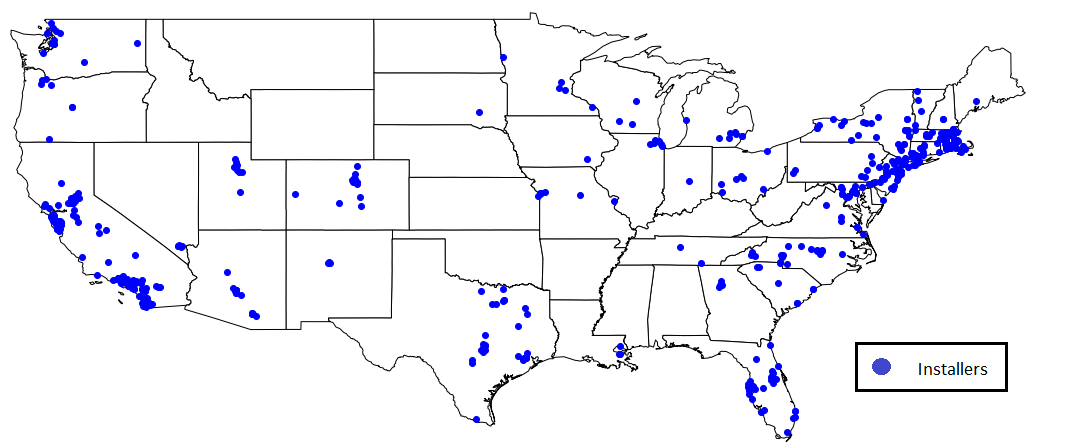
\includegraphics[width=1.1\linewidth]{national_installers.png}
	\caption{Installers in our data set}
	\label{fig:nationalinstallers}
\end{figure}

It is perhaps worth mentioning that based on our conversions with the online marketplace, the marketplace actively reaches out to solar installers to recruit them to join to platform and help them set up their profile. So, unlike starting a physical business, installers' fixed cost of entry to the marketplace is negligibly small (if not zero). This is indeed the case in many different platforms \citep{haddad2015consumer}. In light of this, in this study, we do not study the entry of installers to the marketplace. Rather, we focus on installers' activity levels after they establish their profiles on the marketplace.


%Lastly, we don't observe quitting the platform the same way as physical store closes off. We simply observe inactive profiles. Thus we do not explicitly investigate the exit behavior.





\subsection{Defining Local Market}
\label{defining_local_market}


Solar installation is a combination of product and service. As part of service, installers typically visit the customer site multiple times. Thus, each installer only operates  within a certain geographical area. This means that installers compete ``locally.'' That is, they only compete with installers that are relatively nearby. To capture this practical element, we identify what is called \emph{local markets} within the marketplace so that only installers in the same local market compete with each other.

To geographically segment the marketplace into local markets, we divide installers into multiple \emph{clusters} and treat each cluster as a separate local market. Boundaries of local markets cannot be simply defined by state, county, or congressional district borders because it is common for installers to cross these artificial borders to serve customers. Instead, we use installer locations and the state-of-the-art advanced clustering algorithm called OPTICS (short for \textit{Ordering Points To Identify the Clustering Structure}) to identify local markets.

The OPTICS routine is an unsupervised machine learning algorithm that identifies density-based clusters in spatial data. It is considered to be an extension of various commonly-used advanced clustering algorithms, such as the DBSCAN \citep{kanagala2016comparative}. Among others, an important advantage of the OPTICS algorithm is that it does not require setting the number of clusters before running the algorithm as in $k$-means clustering; rather, it identifies the optimal number of clusters using the data. Because of these advantages, it has been applied in various contexts, ranging from political science \citep{davidson2019neighborhood} to geography \citep{teimouri2016method}.

%data mining \citep{breunig2000fast},

In light of these, we create the geographic division of local markets with the following steps. First, we collected the 5-digit zipcode of
every installer in the marketplace. Figure \ref{fig:nationalinstallers} displays the location of every installer in our data set. We then converted each zipcode  to the representative coordinates based on the data provided by the \citet{us_census_bureau_2019}. This transformation is necessary to run the OPTICS algorithm on the location data. The OPTICS algorithm uses the maximum distance between two samples in a cluster as an input variable. Based on our conversations with the marketplace, we learned that the vast majority of customers get a quote from an installer within 100 miles of their property. We used 90 miles as the maximum distance input parameter to balance between having enough clusters to make use of the inherent variations and making sure that each cluster captures the local market condition. Based on this, the OPTICS algorithm generated 36 clusters.\footnote{We also checked the robustness of our results by taking the maximum distance parameter as 100 miles in the OPTICS algorithm. Our insights remain to be valid in that alternative formulation.} Each of these clusters geographically defines a local market boundary. Figure \ref{fig:markets} illustrates the centroid of each of these 36 clusters, which represents the centroid of each local market. Hereafter, for brevity, we refer to local markets simply as ``\emph{markets}.''



%\paragraph{OPTICS}  The OPTICS algorithm, short for \textit{Ordering Points To Identify the Clustering Structure}, is what we use to cluster installers' coordinates. The OPTICS routine is completed with the following parameter considerations:  \\
%\textbf{min samples: }
%The number of samples in a neighborhood for a point to be considered as a core point.  We use 2 as the default value.
%\textbf{metric}: haversine distance. Although not ideal, it better reflected the distance between two Latitude/Longitude points and is still fast enough in the clustering algorithm.  \textbf{max eps:} The maximum distance between two samples for one to be considered as in the neighborhood of the other. According to the survey that the marketplace conducted, 90.6 percent of customers get a quote from an installer within 100 miles of their property ( 81.7 percent from 50 miles). \citep{marsh_2019} We used 90 as the parameter to balance between having enough clusters to  make use of the inherent variations and make sure each cluster captured the local market condition. We use this cluster to define our market boundary geographically. Figure \ref{fig:markets} illustrates the centroid of each of these 36 clusters, which represents the centroid of each local market. Hereafter, for brevity, we refer to local markets simply as ``\emph{markets}.''



%(PROVIDE A PICTURE TO ILLUSTRATE THE CALINSKI-HARABASZ CURVE VS PARAMETER , refer to figure \ref{optics_parameter_gridsearch} and Calinski-Harabasz criteria : \citep{calinski1974dendrite}.





\begin{figure}
	\centering
	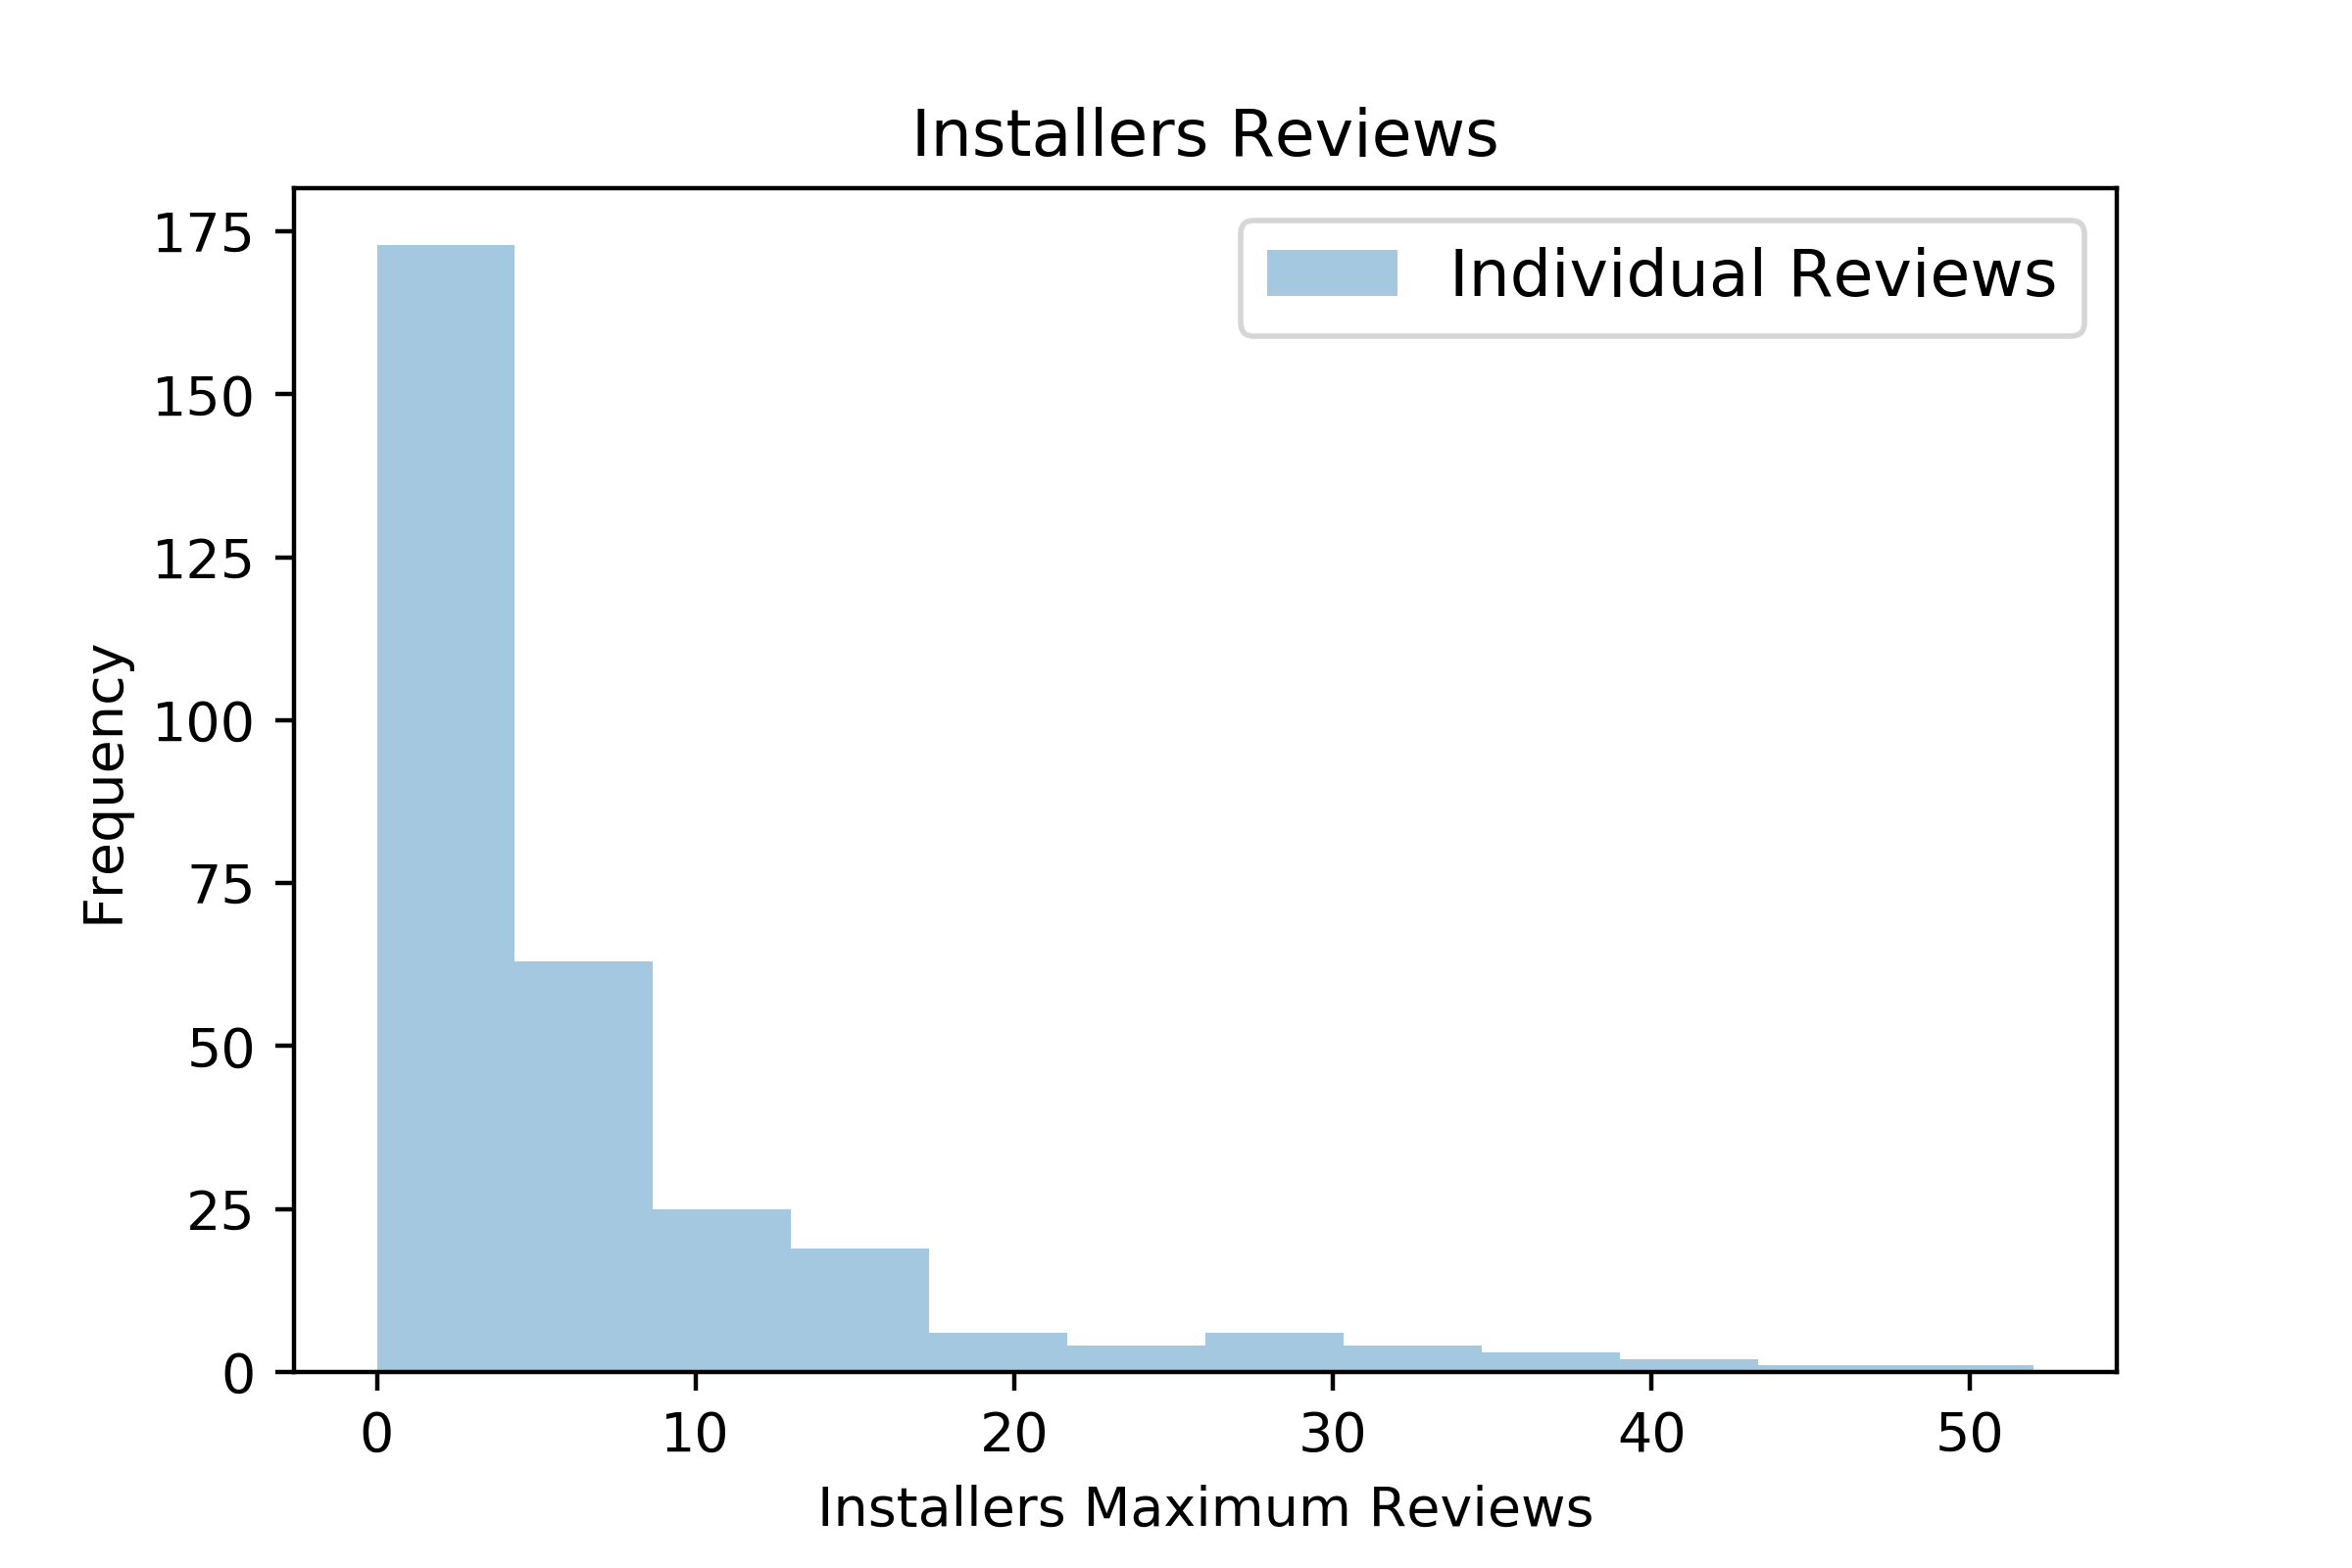
\includegraphics[width=1\linewidth]{histogram_ind_max_reviews_ct.png}
	\caption{Reviews Histogram by Installer}
	\label{histogram_ind_max_reviews_ct}
\end{figure}

% Please add the following required packages to your document preamble:
% \usepackage{booktabs}
\begin{table}
\centering
\begin{tabular}{@{}ccccc@{}}
\toprule
 & Unique  & Total Number & Total Number     & Total Number   \\
State    & Installers & of Reviews   & of Installations & of Quotes \\ \midrule  
CO & 13 & 799  & 168  & 13276 \\
MD & 10 & 895  & 144  & 4054  \\
WA & 9  & 902  & 35   & 1266  \\
TX & 27 & 987  & 90   & 12557 \\
FL & 21 & 994  & 141  & 9047  \\
CT & 10 & 1037 & 78   & 2746  \\
NC & 16 & 1100 & 95   & 7066  \\
NJ & 26 & 1674 & 223  & 8215  \\
NY & 32 & 2790 & 265  & 15128 \\
MA & 36 & 3519 & 507  & 19028 \\
CA & 95 & 7703 & 1472 & 98597 \\ \bottomrule
\end{tabular}
\caption{Top 10 States }
\label{summarystats_top10states}
\end{table}



\begin{figure}
	\centering
	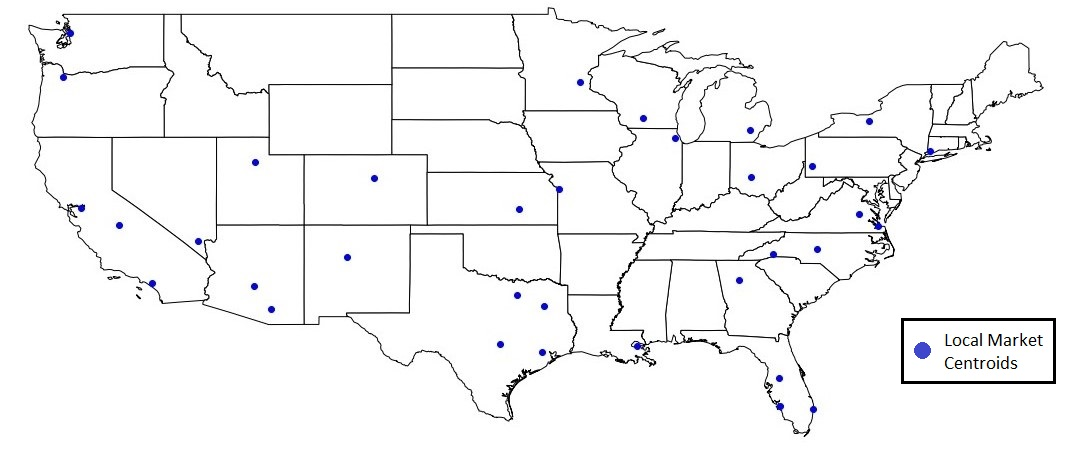
\includegraphics[width=1\linewidth]{markets.jpg}
	\caption{Local Market Centroids}
	\label{fig:markets}
\end{figure}

\subsection{Measuring the Dispersion in Customer Reviews} \label{Subsec: Measure Dispersion}

In our analysis, a key explanatory variable is the dispersion in reviews, which can be measured with numeric ratings (from 1 to 5 stars) or the text content. Below, we first describe how we measure the dispersion of reviews based on ratings. We then explain the innovative word embedding model we use to measure the dispersion of reviews based on the text data. Our base empirical analysis uses the rating-based dispersion as a variable. We then check the robustness of our results by adding the text-based review dispersion as a separate variable in our analysis.

\subsubsection{Measuring Rating-Based Dispersion} \label{Subsec: Define Ent}
We measure the rating-based dispersion by calculating the \emph{entropy} of ratings. In information theory, the entropy is a common way to measure  the uncertainty in a random variable's possible realizations. In our setting, because the marketplace has a 5-star rating system, the entropy of ratings is
\begin{equation}\label{def: entropy}
H(R)=-\sum_{i=1}^{5} \text{Prob}(\text{Rating}=i) \ln(1/\text{Prob}(\text{Rating}=i)).
\end{equation}
For example, for a set of 5 reviews each with 4 stars (out of 5 stars), the entropy of ratings $\{4,4,4,4,4\}$ is zero. Alternatively, for a set of 5 reviews with ratings $\{3,5,3,5,4\}$, the entropy of ratings is 1.0549. Although both sets have the same average rating of 4, the latter set of ratings provides more information with a higher dispersion, hence has a higher entropy.


In light of this, we create three variables that measure the rating entropy in different dimensions for each month $t$. First variable is $\text{Rating\_Entropy\_Self}_{i,t}$ that represents the entropy of each installer $i$'s own reviews. This is calculated on the set of reviews that are associated with installer $i$ up to month $t$. Recalling that market boundaries are defined as in Section \ref{defining_local_market}, the second variable $\text{Rating\_Entropy\_Others}_{i,t}$ that is the rating entropy of all other installers in installer $i$'s market, up to month $t$. In one of our extension sections, we will also consider the rating entropy on the market level. Thus, our third variable is $\text{Rating\_Entropy\_Mkt}_{m,t}$ that represents the entropy of all ratings in the local market $m$, up to that month $t$.  Again, the market is defined as in Section \ref{defining_local_market}.\\

We choose to use entropy to measure the dispersion of ratings over other more common measures, such as variance or coefficient of variance,  for a few practical reasons: 1) The variance has a higher than 0.7 correlation with the average rating. Entropy measures exhibit a lower level of correlation with average ratings. That enabled us to include both variables in the model. 2) entropy measure provides a higher precision (for our data): two installers with very small ratings variance differences tend to show a larger entropy measure difference. \\

\subsubsection{Measuring Text-Based Dispersion via the Language Model BERT} \label{Subsec: Define Txt Ent}

In our analysis, we leverage the rich information in text reviews. To do so, we use the state-of-the-art deep learning based language model called BERT (short for \textit{Bidirectional Encoder Representations from Transformers}). BERT was developed by Google, and published in 2018 \citep{devlin2018bert}. Since then, it has been widely used in practice. For example, Google Search Engine has incorporated this method in October 2019 (REFERENCE). To the best of our knowledge, there is yet no other paper in operations management literature that considers this word embedding technique. We will provide more details about this technique toward the end of this section.

We apply the following steps to measure the text-based dispersion. First, we use the BERT model to convert every piece of review text to a numerical vector. Second, we normalize each vector to unit length. Third, we measure the cosine similarity to find the similarity between every two review vectors. We note that normalization and the cosine similarity measure are standard to identify the similarity between two vectors. See, e.g., \cite{hoberg2016text}. The cosine similarity between two normalized vectors $V_{1}$ and $V_{2}$ equals the inner product of two, i.e.,$V_1 \cdot V_2$, and gives the cosine of the angle between the two vectors. This angle represents the similarity in the orientation of two vectors. If the angle is $0$, the two vectors are at the same orientation and hence the similarity is $1$, which is maximum. After this step, we identify the cosine distance between every two review vectors from the fact that the cosine distance between two normalized vectors $V_{1}$ and $V_{2}$ equals $1$ minus the cosine similarity between the two. This distance reflects how different two reviews are from each other. As the final step, we calculate the dispersion in sets of text reviews, \emph{text-based dispersion}, in short, by enumerating all pairwise distances of reviews in that set and taking their statistical median (the 50th percentile). For example, for a set of 10 text reviews, we have 45 (=$\binom{10}{2}$) pairwise distances. Finding the text-based dispersion for this set requires computing the median distances of these 45 distances. If these 10 pieces of texts are dissimilar from each other, they contain richer information and the median of these $45$ distances shall be higher; and vice versa.

As a result of this procedure, similar to the ratings entropy, we create the following three variables, each measuring the text-based dispersion in a different dimension: (i)$Text\_Dispersion\_Self_{i,t}$: Dispersion in installer $i$'s own text reviews up to month $t$. %Given $N_{i,t}$ pieces of text reviews available up to month $t$, it is calculated by computing $N_{i,t}\times (N_{i,t}-1)/2$ cosine distance pairs and taking the 50$^{th}$ percentile.
(ii) $Text\_Dispersion\_Others_{i,t}$: Dispersion in the text reviews of all other installers in the installer $i$'s local market up to month $t$. %Given $N_{-i,t}$ pieces of text reviews of other installers up to month $t$, it is calculated by computing $N_{-i,t}\times (N_{-i,t}-1)/2$ cosine distance pairs and taking the 50$^{th}$ percentile.
(iii)$Text\_Dispersion\_Mkt_{m,t}$: Dispersion in text reviews of all installers in market $m$ up to month $t$. %Given $N_{m,t}$ reviews available in market $m$ up to month $t$, we calculate $N_{m,t}\times (N_{m,t}-1)/2$ cosine distance pairs and take the 50$^{th}$ percentile to calculate the variable.


We now elaborate the BERT model we used to \textit{vectorize} the text reviews. BERT is a natural language processing (NLP) model that transforms texts into numeric vectors while also preserving the meaning of texts. It belongs to the category of NLP methods called word embedding. In literature, in different contexts than ours, text data are commonly vectorized based on word counts, ignoring the semantics and word ordering (See, e.g., \cite{hoberg2016text} and \cite{loughran2011liability}). However, our context involves texts that are informal writings and often contain emotions. Simply capturing word frequencies does not provide accurate results if similar emotions can be expressed with synonymous words.  Thus, our analysis requires a vectorization that preserves the information and sentiment of the text reviews despite the use of synonyms and/or different styles. The BERT model achieves that. Specifically, the BERT model has two distinct advantages. First, it understands the semantics. For example, consider the 3 sentences:
\begin{align*}
{\footnotesize
\text{Sentence 1: \texttt{they did a good job.}} \quad \text{Sentence 2: \texttt{they did an awful job.}} \quad \text{Sentence 3: \texttt{they did a great job.}}
}
\end{align*}
Considering the meaning of the sentences, we expect the distance between sentences 1 and 3, $D(1,3)$, to be smaller than the distance between 2 and 3 or 1 and 2, i.e., $D(2,3)$ or $D(1,2)$. The BERT model vectorization enables just that; it projects ``good'' and ``great'' to vectors that are closer to each other. In this example, with BERT, we have $D(1,3) = 0.03 < D(1,2) = 0.09 <D(2,3) = 0.1$. This level of distinction is not feasible without word embedding (e.g., by simply using a word counter vectorizer).

Second, the BERT model takes word ordering into account. For example, the two sentences ``The food was good, not bad at all'' and ``The food was bad, not good at all'' have the opposite meaning. Common vectorization methods (e.g., ``bag-of-words'' approach) are not able to capture this difference as words and number of counts are the same in both sentences. But, the BERT model can easily differentiate between these two sentences.


\section{Installer-Level Analysis \& Results} \label{Sec: Installer-level}

This section answers the following two questions: (i) How does the dispersion in an installer's reviews impact the  number of proposals generated by the installer, which is referred to as the installer's \emph{activity level}. (ii) How does the dispersion in competitor installers' reviews impact the installer's activity level?

To answer these questions, we run a regression model where the response variable is $Installer\_Activity_{i,m,t}$ and calculated as $\log$(proposals generated by installer $i$ + 1) in the market $m$ during month $t$. In our regression, first, we only use numerical ratings. Later, as a separate analysis, we will use text-based dispersion variables in our regression.

\subsection{Model \& Controls}

Recalling the entropy variables defined in Section \ref{Subsec: Define Ent}, we run the following regression model on our panel data:
\begin{align}  \nonumber
    \text{Installer\_Activity}_{i,m,t+1}=&\beta_{0}+\beta_{1} \text{Rating\_Entropy\_Self}_{i,t}+\beta_{2} \text{Rating\_Entropy\_Self}_{i,t}^ {2}
    \\ \nonumber
    &+\beta_{3} \text{Rating\_Entropy\_Others}_{i,t}  +\beta_{4}\text{Rating\_Entropy\_Others}_{i,t}^{2} \\ \label{model_ind_3}
    &+ \text{Controls}_{i,m,t}+ \alpha_{i} + \epsilon_{i,t+1}.
\end{align}
 Here, $\epsilon$ is the installer-level error term, and represents random factors that are unobservable in the data and affect the installer activity.


 We run two versions of \eqref{model_ind_3}: In one version, we consider $\alpha_{i}$ as a fixed effect whereas in the alternative version, we consider it as a random effect. To determine which model is more appropriate for our data, we run the Durbin-Wu-Hausman test where the null hypothesis is that the the random-effect model is preferred while the alternative is the fixed-effect model. With a p-value $<0.0001$, we reject the null hypothesis and conclude that the fixed-effect model is more appropriate. We also establish the significance of the fixed effect in \eqref{model_ind_3} with the $F$-test. Thus, we focus on \eqref{model_ind_3} with the installer-level fixed effect $\alpha_{i}$ that controls for time-invariant characteristics of each installer.


 The regression \eqref{model_ind_3} includes various additional installer-level or market-level control variables ($\text{Controls}_{i,m,t}$). To account for the state-level renewable policy effects, we include state dummies denoted by ``State'' as a control variable. We have 33 such variables. We account for the impact of the solar panel prices on installers' activities by considering $\text{Price\_Difference}_{i,t}$ as another control variable. We use the TTS data to find each installer's price for 1 KW solar panel via matching name and zipcode. In practice, price per KW is a common way to assess the price of a solar panel as solar systems vary in size. Based on this, we compute the variable $\text{Price\_Difference}_{i,t}$ as taking the logarithm of the difference between installer $i$'s price and the average price of its competitors that operate in the same market in month $t$.  We control for the self average rating of each installer $i$ $\text{Avg\_Rating\_Self}_{i,t}$  as well as the average ratings of its competitors $\text{Avg\_Rating\_Others}_{i,t}$ in the market for month $t$. We also control for the experience of the installer by considering the variable $\text{Experience}_{i,t}$ that is the logarithm of number of years the installer has been installing solar systems up to month $t$. We obtain this information from each installer's website. Another control variable in \eqref{model_ind_3} is $\text{Market\_Revenue}_{m,t}$  that measures the total dollar value of all solar installations within market $m$ during month $t$. To create this variable, we augment the market boundaries identified in Section \ref{defining_local_market} with the TTS data to capture total  solar installations opportunities in the market. Finally, we consider the count of each installer $i$'s self reviews up to (and including) month $t$, and denote it by $\text{Review\_Counts}_{i,t}$.





% the following regression equation is used to estimate the impact of ratings dispersion (own ratings dispersion: $Ent_{i,self,t}$ ; others ratings dispersion: $Ent_{i,others,t}$) on focal installer's activity intensities $ActInt_{i,m,t}$:
%\begin{equation}
%    ActInt_{i,m,t+1}=\beta_{0}+\beta_{11} Ent_{i,m,others,t}+\beta_{2}Ent_{i,m,others,t}^2+
%   Controls_{i,t}+\alpha_{i}+\epsilon_{i,m,t}
%   \label{model_ind_1}
%\end{equation}
%
%\begin{equation}
%    ActInt_{i,m,t+1}=\beta_{3}+\beta_{4} Ent_{i,self,t}+\beta_{5}Ent_{i,self,t}^2+
%   Controls_{it}+\alpha_{i}+\epsilon_{i,m,t}
%   \label{model_ind_2}
%\end{equation}

Tables \ref{sumstats_ind} and \ref{corr_ind} below present the summary statistics and the correlation matrix. By Table \ref{corr_ind}, correlations are in the expected direction and do not hurt the validity of regression analysis.

% Please add the following required packages to your document preamble:
% \usepackage{booktabs}
% \usepackage{graphicx}
\begin{table}[H]
\centering
\begin{tabular}{@{}lccccc@{}}
\toprule
Variables               & N     & Mean    & Standard Deviation & Min    & Max   \\ \midrule
Rating\_Entropy\_Self   & 4,562 & 0  & 0.217  & -0.0985 & 0.9015     \\
Rating\_Entropy\_Others & 4,562 & 0   & 0.183  & -0.227  & 0.773     \\
Average\_Rating\_Self   & 4,562 & 4.531   & 1.316  & 1      & 5     \\
Average\_Rating\_Others & 4,562 & 4.88    & 0.205  & 1      & 5     \\
Review\_Count           & 4,562 & 5.384   & 6.836  & 0      & 52    \\
Experience              & 4,562 & 1.758   & 0.929  & 0      & 3.714 \\
Price\_Difference       & 4,562 & -0.0333 & 0.392  & -2.171 & 3.139 \\
Market\_LogRevenue      & 4,562 & 12.24   & 7.9    & 0      & 22.3  \\ \bottomrule
\end{tabular}%
\caption{Summary Statistics - Installer Level Analysis}
\label{sumstats_ind}
{\footnotesize \textit{Note: All entropy variables are demeaned.}}
\end{table} 

% Please add the following required packages to your document preamble:
% \usepackage{booktabs}
% \usepackage{graphicx}
\begin{table}[H]
\centering
\begin{tabular}{@{}lllllllll@{}}
\toprule
Variables                   & (1)    & (2)    & (3)    & (4)    & (5)    & (6)    & (7)        & (8)     \\ \midrule
(1) Rating\_Entropy\_Self   & 1      & \multicolumn{7}{l}{}                                              \\
(2) Rating\_Entropy\_Others & -0.094 & 1      & \multicolumn{6}{l}{}                                     \\
(3) Average\_Rating\_Self   & -0.088 & 0.069  & 1      & \multicolumn{5}{l}{}                            \\
(4) Average\_Rating\_Others & 0.025  & -0.523 & -0.017 & 1      & \multicolumn{4}{l}{}                   \\
(5) Review\_Count           & 0.241  & 0.061  & 0.205  & -0.039 & 1      & \multicolumn{3}{l}{}          \\
(6) Experience              & -0.001 & 0.143  & 0.036  & -0.062 & 0.127  & 1      & \multicolumn{2}{l}{} \\
(7) Price\_Difference       & -0.015 & -0.043 & 0.003  & 0.016  & -0.029 & -0.027 & 1          &         \\
(8) Market\_LogRevenue      & -0.026 & 0.006  & -0.029 & 0.044  & -0.086 & 0.451  & -0.059     & 1       \\ \bottomrule
\end{tabular}%
\caption{Correlation Matrix - Installer Level Analysis}
\label{corr_ind}
\end{table} 

\subsection{Results}

Table \ref{reg_ind_all} presents results estimated by three panel regression models based on \eqref{model_ind_3}. Columns (1) through (3) of Table \ref{reg_ind_all} correspond to results obtained by using different set of explanatory variables in the regression. The results in the column (3) correspond to the ones estimated by \eqref{model_ind_3}; others are estimated by considering only some of these variables in the regression. In particular, column (1) corresponds to results when entropy variables are not considered at all whereas column (2) are the estimates when we include only others' entropy ( $\text{Rating\_Entropy\_Others}\_{i,t}$).


% Please add the following required packages to your document preamble:
% \usepackage{booktabs}
% \usepackage{graphicx}
\begin{table}[]
\centering
\begin{threeparttable}
\begin{tabular}{@{}lccc@{}}
\toprule
                  & (I)      & (II)    & (III)   \\  
& Installer's Activity & Installer's Activity & Installer's Activity \\
Variables & Level    & Level   & Level   \\ \midrule
Rating\_Entropy\_Self                                &                            &                            & 1.890***                   \\
                                                     &                            &                            & (0.000)                    \\
Rating\_Entropy\_Self$^2$                            &                            &                            & -3.473***                  \\
                                                     &                            &                            & (0.000)                    \\
Rating\_Entropy\_Others                              &                            & 0.524**                    & 0.488**                    \\
                                                     &                            & (0.004)                    & (0.007)                    \\
Rating\_Entropy\_Others$^2$                          &                            & -2.533***                  & -2.593***                  \\
                                                     &                            & (0.000)                    & (0.000)                    \\
Average\_Rating\_Self                                & -0.876***                  & -0.834***                  & -0.774**                   \\
                                                     & (0.000)                    & (0.000)                    & (0.001)                    \\
Average\_Rating\_Others                              & 0.000618                   & 0.000236                   & 0.000964                   \\
                                                     & (0.975)                    & (0.991)                    & (0.963)                    \\
Review\_Count                                        & 0.0561***                  & 0.0534***                  & 0.0472***                  \\
                                                     & (0.000)                    & (0.000)                    & (0.000)                    \\
Experience                                           & 0.218***                   & 0.212***                   & 0.206***                   \\
                                                     & (0.000)                    & (0.000)                    & (0.000)                    \\
Price\_Difference                                    & 0.0593                     & 0.0690                     & 0.0722                     \\
                                                     & (0.487)                    & (0.425)                    & (0.402)                    \\
Market\_LogRevenue                                   & -0.0168***                 & -0.0169***                 & -0.0159***                 \\
                                                     & (0.000)                    & (0.000)                    & (0.001)                    \\
Constant                                             & 2.690***                   & 2.803***                   & 2.961***                   \\
                                                     & (0.000)                    & (0.000)                    & (0.000)                    \\
Observations                                         & 4562                       & 4562                       & 4562                       \\
Fixed Effect                             & Yes        & Yes        & Yes       \\
State Dummies                            & Yes        & Yes        & Yes       \\
Adjusted R$^2$                                                     & 0.627                      & 0.630                      & 0.633       \\
AIC                                                  & 13267.2                    & 13234.9                    & 13205.7                    \\
BIC                                                  & 13325.0                    & 13305.6                    & 13289.2                    \\ \bottomrule

\end{tabular}%
\begin{tablenotes}
\item Note: $p$-value in parentheses; $^\star p<0.05;^{\star\star} p<0.01;^{\star\star\star} p<0.001 $
\end{tablenotes}
\caption{Installer Level Analysis}
\label{reg_ind_all}
\end{threeparttable}
\end{table}

Our estimates in Table \ref{reg_ind_all} identify three key results. First, the set of variables representing ``noise'' or dispersion of ratings have a significant impact on the activity level of an installer in the marketplace. Second, the entropy of an installer's own ratings has a positive and statistically significant effect on its activity level (because $\beta_{1}$ in equation \eqref{model_ind_3} is found to be positive and significant in column(3) of Table \ref{reg_ind_all}), and the second-order effect ($\beta_{2}$ in equation \eqref{model_ind_3})) of an installer's ratings entropy is negative and statistically significant. Combining these two effects, the regression estimates indicate that the dispersion of an installer's own ratings increases the installer's activity level if and only if the aforementioned dispersion is small. When the dispersion of its own ratings is large, any additional dispersion in the installer's own ratings deters the its activity in the marketplace.

Third and most important, our estimation shows that the entropy of competitor ratings impacts an installer's activity level in the \emph{same} way as the entropy of the installer's own ratings. That is, the dispersion of competitor ratings increases the installer's activity level if and only if the aforementioned dispersion is small. When the dispersion of competitor ratings is large, any additional dispersion in competitor ratings deters the installer's activity in the marketplace.


Figures \ref{fig: marginsplot_ind_ent_self} and  \ref{fig: marginsplot_ind_ent_others} illustrate the explained non-linear effects of the rating entropy on installer's activity level. To generate the marginal effects displayed in Figures \ref{fig: marginsplot_ind_ent_self} and  \ref{fig: marginsplot_ind_ent_others}, we use the estimated regression coefficients in the column (3) of Table \ref{reg_ind_all}. As is apparent from these figures, the installer's activity level first increases then decreases with the rating dispersion, and that is true regardless of whether installer's own ratings or its competitors' ratings are considered.

\begin{figure}
	\centering
	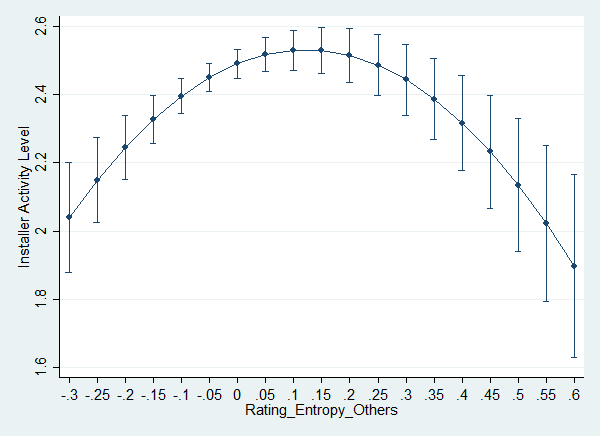
\includegraphics[width=0.7\linewidth]{marginsplot_entothers.png}
	\caption{Marginal Impact of the Entropy of Other Installers' Ratings (in the same market) on the Installer's Activity Level}
	\label{fig: marginsplot_ind_ent_others}
\end{figure}



\begin{figure}
	\centering
	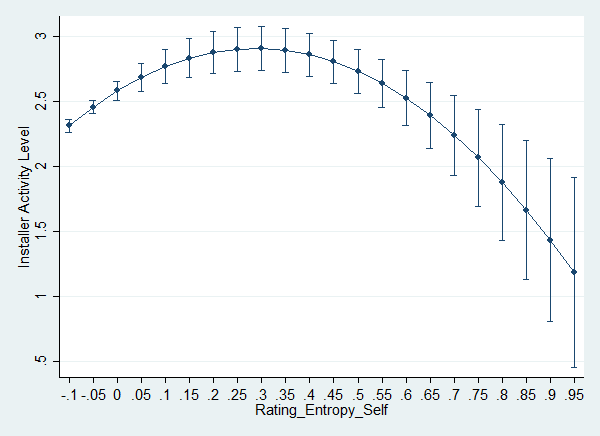
\includegraphics[width=0.7\linewidth]{marginsplot_entself.png}
	\caption{Marginal Impact of the Entropy of the Installer's Own Ratings on its Activity Level}
	\label{fig: marginsplot_ind_ent_self}
\end{figure}


Finally, it might be worth noting that in the first two columns average of own or others ratings did not appear to be significantly linked with activity intensity levels. Yet after we controlled for dispersion, we noticed a negative effect associated with installers' own average. Installers appear to extend fewer proposals as their own ratings increase, after all other factors are controlled for. We think this is a phenomenon that installers are more selective after they attained a high rating on the platform, perhaps acting out of confidence that with a higher rating, their proposals are more likely to be accepted by customers.

\section{Market-Level Analysis \& Results} \label{Sec: Market-level}

An important performance metric for the marketplace is the number of matches (i.e., agreed proposals) between installers and customers on the marketplace. This section estimates how the dispersion of ratings in a market impacts the number of matches in that market.

For this estimation, we use the regression equation in \eqref{reg: market-level-rating}. Our data include the number of agreed proposals for each installer $i$ in each month $t$. To create our dependent variable $\text{Market\_Transaction}_{m,t+1}$, we first calculate the total number of proposals accepted by customers in market $m$ and month $t+1$, and then take logarithmic transformation of that sum. Formally, $\text{Market\_Transaction}_{m,t+1} =$ $\ln\left( \sum_{i \in \text{Market\ } m} \text{Successful\_Proposals}_{i}+ 1 \right)$.  With this, we convert the installer-level monthly panel data to market-level monthly panel data so that we can exploit the market-level rating dispersion to identify its impact on the local market outcome.
\begin{align} \nonumber
   Market\_Transaction_{m,t+1} & =\beta_{5} + \beta_{6} Rating\_Entropy\_Mkt_{m,t}+ \beta_{7} Rating\_Entropy\_Mkt_{m,t} ^2\\ \label{reg: market-level-rating}
   &+ Controls_{m,t}  +\epsilon_{m,t+1}.
\end{align}

Here, $Rating\_Entropy\_Mkt_{m,t}$ is as defined in Section \ref{Subsec: Define Ent} and equals the entropy of ratings up to (and including) month $t$ from all installers in the market $m$.

We also use various control variables denoted by $\text{Controls}_{m,t}$. We control for the state of the market. We created 33 state dummies to represent 33 different state represented in the data set. Some market span across more than one state. In that case, we calculated state representation fractions and assign its value (between 0 to 1) to the state indicator variable ( i.e.  market 1 has 25\% of installers from state CA and 75\% from NV, then we assign 0.25 to dummy STATE\_CA and 0.75 to dummy STATE\_NV). Similar to the installer-level analysis in Section \ref{Sec: Installer-level}, we created the $\text{Avg\_Experience}_{m,t}$ variable to represent the average experience of installers in the market $m$ up to and including month $t$. We calculated this by averaging installers' experiences level across the local market $m$. In parallel to the installer-level analysis, we use the $\text{Avg\_Rating\_Mkt}_{m,t}$ to control for the average rating of all installers in the market $m$ until (and including) month $t$. As another control, we created $\text{Review\_Count\_Mkt}_{m,t}$ that measures the total number of reviews by all installers in market $m$ up to and including month $t$. We also control for the difference of average unit price between marketplace and off-marketplace. We use $\text{Price\_Diff\_Mkt}_{m,t}$ to denote this variable. Finally, we use $\text{Market\_Revenue}_{m,t}$ as a control where it is as defined in Section \ref{Sec: Installer-level}.Summary statistics can be found in Table \ref{sumstats_mkt}; the correlation coefficients among variables are presented in Table \ref{corr_mkt}.

\subsection{Results}


The results are presented in Table \ref{reg_mkt_simplified}. Column (1) are the estimates obtained by running the regression in \eqref{reg: market-level-rating} in the absence of $\text{Rating\_Entropy\_Mkt}_{m,t}$ and $\text{Rating\_Entropy\_Mkt}^2_{m,t}$ variables, and  Column (2) are the estimates obtained by running the regression in \eqref{reg: market-level-rating} considering all variables in \eqref{reg: market-level-rating}.
% Please add the following required packages to your document preamble:
% \usepackage{booktabs}
% \usepackage{graphicx}
\begin{table}[H]
\centering

\begin{tabular}{@{}lccccc@{}}
\toprule
Variables            & N   & Mean   & Standard Deviation & Min    & Max   \\ \midrule
Rating\_Entropy\_Mkt & 642 & 0  & 0.236              & -0.191  & 0.809    \\
Market\_LogRevenue   & 642 & 7.887  & 8.102               & 0      & 22.3  \\
Average\_Rating\_Mkt & 642 & 4.870  & 0.245              & 3      & 5     \\
Average\_Experience  & 642 & 1.426 & 1.110              & 0      & 3.332    \\
Price\_Difference\_Mkt    & 642 & -0.0106 & 0.146              & -0.504 & 1.312 \\ \bottomrule
\end{tabular}%

\caption{Summary Statistics - Market Level Analysis}
\label{sumstats_mkt}
\end{table} 
% Please add the following required packages to your document preamble:
% \usepackage{booktabs}
% \usepackage{graphicx}
\begin{table}[H]
\centering
\begin{tabular}{@{}llllll@{}}
\toprule
Variables                & (1)    & (2)    & (3)    & (4)    & (5) \\ \midrule
(1) Rating\_Entropy\_Mkt & 1      &        &        &        &     \\
(2) Average\_Rating\_Mkt & -0.624 & 1      &        &        &     \\
(3) Average\_Experience  & 0.198  & -0.107 & 1      &        &     \\
(4) Price\_Difference\_Mkt    & -0.018 & -0.041 & -0.012 & 1      &     \\
(5) Market\_LogRevenue   & 0.157  & -0.041 & 0.498  & -0.126 & 1   \\ \bottomrule
\end{tabular}
\caption{Correlation Matrix - Market Level Analysis}
\label{corr_mkt}
\end{table} 
% Please add the following required packages to your document preamble:
% \usepackage{booktabs}
% \usepackage{graphicx}
\begin{table}[]
\centering
\begin{threeparttable}[t]
\begin{tabular}{@{}lcc@{}}
\toprule
                                    & (I)                   & (II)                  \\
Variables                                    & Market Transaction & Market Transaction\\ \midrule
Rating\_Entropy\_Mkt                         &                       & 1.060***              \\
                                             &                       & (0.000)               \\
Rating\_Entropy\_Mkt$^2$                     &                       & -1.610***             \\
                                             &                       & (0.000)               \\
Average\_Rating\_Mkt                         & -0.273                & -0.185                \\
                                             & (0.071)               & (0.212)               \\
Average\_Experience                          & 0.0197*               & 0.0138                \\
                                             & (0.013)               & (0.073)               \\
Price\_Difference\_Mkt                       & 0.239                 & 0.287                 \\
                                             & (0.282)               & (0.194)               \\
Market\_LogRevenue                           & -0.0846               & -0.0663               \\
                                             & (0.057)               & (0.123)               \\
Constant                                     & 3.443**               & 2.909*                \\
                                             & (0.009)               & (0.025)               \\
Market Fixed Effect                          & Yes                   & Yes                   \\
Weighted State Dummies                       & Yes                   & Yes                   \\
Observations                                 & 642                   & 642                   \\
Adjusted R$^2$                                  & 0.739                 & 0.747                 \\
AIC                                          & 1075.6                & 1059.6                \\
BIC                                          & 1156.0                & 1148.9                \\ \bottomrule
\end{tabular}%
\begin{tablenotes}
\item Note: $p$-value in parentheses; $^\star p<0.05;^{\star\star} p<0.01;^{\star\star\star} p<0.001 $
\end{tablenotes}
\caption{Market Level Analysis}
\end{threeparttable}
\label{reg_mkt_simplified}
\end{table} 



he ``noise'' portion of the ratings remains a significant factor. The estimate suggest that on the market level reviews dispersion is directly linked to higher number of total matches (proposals accepted), as reflected in the positive and statistically significant coefficient ($\beta_{5}=1.628,p<0.01$ ). We also note that the second order effect is negative as the coefficient estimates associated with the square term is negative ($\beta_{6}=-1.160,p<0.01$) and statistically significant. Combining these two effects, the regression estimates indicate that the dispersion of installers ratings on a local market increases the local market matches if and only if the aforementioned dispersion is small. When the dispersion of market level ratings is large, any additional dispersion in the market level dampens the market level matching activity.\\
We further illustrate this point with a margins plot using coefficients generated from estimates in column (2) of table \ref{reg_mkt_simplified} in figure \ref{fig: marginsplot_mkt_entmkt}. As it is apparent from this figure, the market level matching increase then decreases with the ratings dispersion.\\

Finally, the results on the local market level also suggest that after controlling for local market conditions, installer experience, price, and state, the average rating is not significantly associated with the market level performance.
\begin{figure}
	\centering
	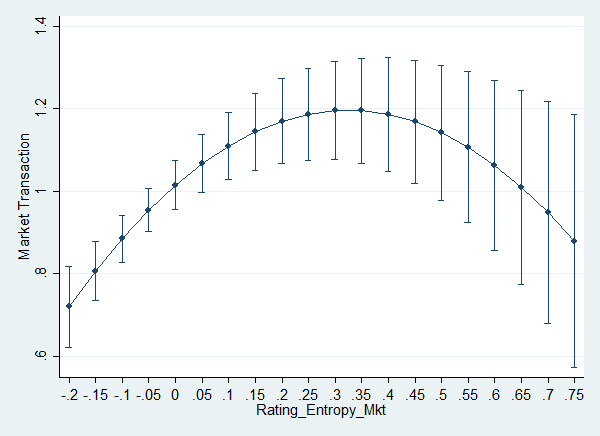
\includegraphics[width=0.7\linewidth]{marginsplot_entmkt.png}
	\caption{Marginal Impact of Market Reviews Entropy of Reviews on Market Level Matching}
	\label{fig: marginsplot_mkt_entmkt}
\end{figure}







\section{Text Mining}
% Please add the following required packages to your document preamble:
% \usepackage{booktabs}
% \usepackage{graphicx}
\begin{table}[H]
\centering
\begin{threeparttable}[t]
\begin{tabular}{@{}lcccc@{}}
\toprule
                            & (I)         & (II)        & (III)       & (IV)        \\
                            & Installer's & Installer's & Installer's & Installer's \\
Variables                   & Activity Level & Activity Level & Activity Level & Activity Level \\ \midrule
Text-based\_Entropy\_Self   & 5.326***    & 5.389***    & 5.014***    & 4.890***    \\
                            & (0.000)     & (0.000)     & (0.000)     & (0.000)     \\
Text-based\_Entropy\_Self$^2$    & -23.71***           & -23.54***              & -20.29***      & -20.40***      \\
                            & (0.000)     & (0.000)     & (0.000)     & (0.000)     \\
Text-based\_Entropy\_Others & -1.288      & -0.989      & -1.640      & -1.955      \\
                            & (0.389)     & (0.509)     & (0.275)     & (0.193)     \\
Text-based\_Entropy\_Others$^2$   & -9.593              & -13.13                 & 1.348          & 5.132          \\
                            & (0.623)     & (0.517)     & (0.944)     & (0.782)     \\
Average\_Rating\_Self       & -0.942***   &             &             & -0.998***   \\
                            & (0.000)     &             &             & (0.000)     \\
Average\_Rating\_Others     & 0.000219    &             &             & -0.00483    \\
                            & (0.991)     &             &             & (0.813)     \\
Average\_Sentiment\_Self    &             & -0.431      & -0.404      &             \\
                            &             & (0.090)     & (0.129)     &             \\
Average\_Sentiment\_Others  &             & 0.111       & 0.0806      &             \\
                            &             & (0.378)     & (0.524)     &             \\
Rating\_Entropy\_Self       &             &             & 2.044***    & 2.161***    \\
                            &             &             & (0.000)     & (0.000)     \\
Rating\_Entropy\_Self$^2$              &                     &                        & -4.246***      & -4.344***      \\
                            &             &             & (0.000)     & (0.000)     \\
Rating\_Entropy\_Others     &             &             & 0.399*      & 0.384*      \\
                            &             &             & (0.033)     & (0.045)     \\
Rating\_Entropy\_Others$^2$          &                     &                        & -2.382***      & -2.376***      \\
                            &             &             & (0.000)     & (0.000)     \\
Review\_Count               & 0.0489***   & 0.0492***   & 0.0420***   & 0.0413***   \\
                            & (0.000)     & (0.000)     & (0.000)     & (0.000)     \\
Experience                  & 0.178***    & 0.175***    & 0.176***    & 0.177***    \\
                            & (0.001)     & (0.001)     & (0.001)     & (0.001)     \\
Price\_Difference           & 0.0952      & 0.101       & 0.125       & 0.118       \\
                            & (0.278)     & (0.247)     & (0.158)     & (0.181)     \\
Market\_LogRevenue          & -0.0164***  & -0.0165***  & -0.0159***  & -0.0158***  \\
                            & (0.000)     & (0.000)     & (0.001)     & (0.001)     \\
Constant                    & 2.374***    & 2.075***    & 2.379***    & 2.649***    \\
                            & (0.000)     & (0.000)     & (0.000)     & (0.000)     \\
Fixed Effect                & Yes        & Yes         & Yes          &Yes \\
State Dummies               & Yes        & Yes        & Yes           &Yes\\                          
Observations                & 4562        & 4562        & 4562        & 4562        \\
Adjusted-R$^2$                          & 0.633       & 0.633       & 0.638       & 0.638       \\
AIC                         & 13202.7     & 13200.9     & 13147.9     & 13147.6     \\
BIC                         & 13292.7     & 13290.8     & 13263.5     & 13263.2     \\ \bottomrule
\end{tabular}%
\begin{tablenotes}
\item Note: $p$-value in parentheses; $^\star p<0.05;^{\star\star} p<0.01;^{\star\star\star} p<0.001$
\end{tablenotes}
\end{threeparttable}
\caption{Installer Level Analysis with Variables Derived from Text Analysis}
\label{reg_ind_withtext}
\end{table} 
% Please add the following required packages to your document preamble:
% \usepackage{booktabs}
% \usepackage{graphicx}
\begin{table}
\centering
\begin{threeparttable}
\begin{tabular}{@{}lccc@{}}
\toprule
                                               & (I)            & (II)           & (III)          \\
                                               & Market    & Market    & Market    \\
Variables                                      & Transaction & Transaction & Transaction \\ \midrule
Rating\_Entropy\_Mkt                         &                       &                       & 1.605***              \\
                                             &                       &                       & (0.000)               \\
Rating\_Entropy\_Mkt$^2$ &                       &                       & -1.622***             \\
                                             &                       &                       & (0.000)               \\
Average\_Rating\_Mkt                         & -0.259                &                       &                       \\
                                             & (0.092)               &                       &                       \\
Average\_Sentiment\_Mkt                      &                       & -1.316**              & -1.180*               \\
                                             &                       & (0.006)               & (0.012)               \\
Average\_Experience                          & 0.0193*               & 0.0148                & 0.00983               \\
                                             & (0.016)               & (0.058)               & (0.196)               \\
Price\_Difference\_Mkt                       & 0.228                 & 0.228                 & 0.292                 \\
                                             & (0.314)               & (0.301)               & (0.182)               \\
Market\_LogRevenue                           & -0.0820               & -0.0652               & -0.0517               \\
                                             & (0.066)               & (0.125)               & (0.214)               \\
Text\_Dispersion\_Mkt                        & 3.014                 & 1.318                 & -1.856                \\
                                             & (0.443)               & (0.736)               & (0.632)               \\
Text\_Dispersion\_Mkt$^2$                    & -7.258                & -3.138                & 3.539                 \\
                                             & (0.420)               & (0.730)               & (0.691)               \\
Constant                                     & 3.124*                & 2.843*                & 2.688*                \\
                                             & (0.024)               & (0.017)               & (0.021)               \\
Fixed Effect                                   & Yes            & Yes            & Yes            \\
State Dummies                                  & Yes            & Yes            & Yes            \\
Observations                                 & 642          & 642          & 642                  \\
Adjusted R$^2$                               & 0.739                 & 0.743                 & 0.750                 \\
AIC                                            & 8853.4         & 8849.3         & 8843.7         \\
BIC                                            & 8925.9         & 8933.9         & 8928.3         \\ \bottomrule
\end{tabular}%
\begin{tablenotes}
\item Note: $p$-value in parentheses; $^\star p<0.05;^{\star\star} p<0.01;^{\star\star\star} p<0.001$
\end{tablenotes}
\end{threeparttable}
\caption{Market Level Analysis with Variables Derived from Text Analysis}
\label{reg_mkt_textbased}
\end{table} 
In this section, we incorporate various methods to leverage the rich text information in reviews.  We first use NLP method to generate sentiment score of each reviews. We also apply BERT model to perform word embedding, and generated measures for texts dispersion. We replace quantitative metrics derived from ratings with text mining measures in our analysis.

\subsection{Sentiment Score of reviews Texts}
In this section, we introduce methods to generate sentiment scores on the reviews texts. We use VADER model to generate text sentiment score. VADER, developed by  \cite{hutto2014vader} as a `Parsimonious Rule-Based Model for Sentiment Analysis of Social Media Text'. Since reviews texts shares many stylistic similarities with social media text, this is an appropriate approach. For a piece of text, the language model produces a compound sentiment score from -1 to 1, with 1 representing very positive and -1  very negative sentiments.


Example 1:

\textit{Mike at (...) was friendly, courteous, professional and very helpful.  At first I did not know what kind of system I wanted, because my roof was too small and I had some trees in the way.  Mike had never installed a tracking system but he did recommend it.  It seemed like we would get the best "bang for the buck" with this system, so I went with it.  Mike had all subcontractor there on time as well as all the equipment.  It was up and running in less than a week.  I love it.}

The above review received a compound sentiment score of 0.8622 and a five-star rating. \\
Example 2:

\textit{Do not hire (...)  to install a solar system. Do not hire (...) to do anything. Evan   and all his various companies and names  ARE NOT LICENCED OR INSURED. I was scammed by Mr. Evan (...) in December of 2013. He installed the system wrong and incomplete even though all the parts and materials were provided for him. Please take the time to do your research and check references and validate licenses and insurance information. It will save u more money than to trust a cheap con artist. All the info at (...)  is fraudulent lies. Evan Esposito is also known as (...).}

This received -0.7184 sentiment score and an one-star rating.

\subsection{Analysis using Variables Derived From Text Mining}
We move on to discuss the analysis which we conduct with variables derived from text mining. We have introduced two models BERT and VADER which are used for construct dispersion and average sentiment measures, respectively. Overall, the sentiment score correlates with ratings significantly(corr = 0.8239), while the text-based dispersion measure correlates with the entropy measures on a lower level (corr = 0.4309). The correlation between sentiment score and ratings is further illustrated in figure \ref{sent_score_scatter} with a violinplot. And for the relationship between text-based dispersion and ratings entropy, we present a scatter plot with a regression line in figure \ref{fig: regplot_text_d_ent_others}. \\
We are interested to determine if installers and market level activities can also be attributed to sentiment scores and text-based dispersion measures. We use variables $\text{Avg\_Sent\_Self}_{i,t}$ in place of $\text{Avg\_Rating\_Self}_{i,t}$, $\text{Avg\_Sent\_Others}_{i,m,t}$ in place of $\text{Avg\_Others}_{i,m,t}$ to represent individual ratings in individual level analysis, $\text{Avg\_Sent\_Mkt}_{m,t}$ in place of $\text{Avg\_Mkt}_{m,t}$ in market level analysis, and ran the same regression models. The results are presented in table \ref{reg_ind_withtext} for installer level analysis and table \ref{reg_mkt_textbased} for market level analysis.  \\
In table \ref{reg_ind_withtext}, column (1) through (4) contains results obtained by using different set of explanatory variables. Specifically, (1) and (2) contains results including only $\text{Text\_Based\_Dispersion\_Others}$, where column (1) model uses average ratings and column (2) model uses average sentiment score. Moving on, the models used in column (3) and (4) have a parallel structure, but included installers' own text-based dispersion.  \\

We observe the same type of inverse U shape for the marginal impact of text-based dispersion. \\

\begin{align}  \nonumber
    \text{Installer\_Activity}_{i,m,t+1}=&\beta_{0}+\beta_{1} \text{Text\_Dispersion\_Self}_{i,t}+\beta_{2} \text{Text\_Dispersion\_Self}_{i,t}^ {2}
    \\ \nonumber
    &+\beta_{3} \text{Text\_Dispersion\_Others}_{i,t}  +\beta_{4}\text{Text\_Dispersion\_Others}_{i,t}^{2} \\ \label{model_ind_textbased}
    &+ \text{Controls}_{i,m,t}+ \alpha_{i} + \epsilon_{i,t+1}.
\end{align}

\begin{align}
   \text{Market\_Transaction}_{m,t+1}  =\beta_{5} + \beta_{6}\text{Text\_Dispersion\_Mkt}_{m,t}+ \\ \nonumber \beta_{7} \text{Text\_Dispersion\_Mkt}_{m,t} ^2 \label{reg: market-level-textbased}
   &+ Controls_{m,t}  +\epsilon_{m,t+1}.
\end{align}
\begin{figure}
	\centering
	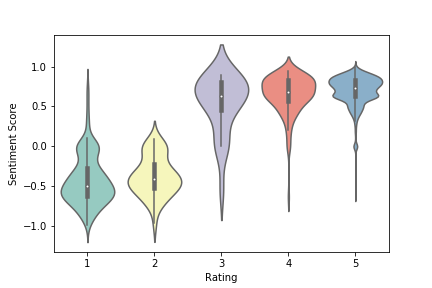
\includegraphics[width=0.7\linewidth]{sentscore_violin.png}
	\caption{Sentiment Scores and Ratings}
	\label{sent_score_scatter}
\end{figure}
\begin{figure}
	\centering
	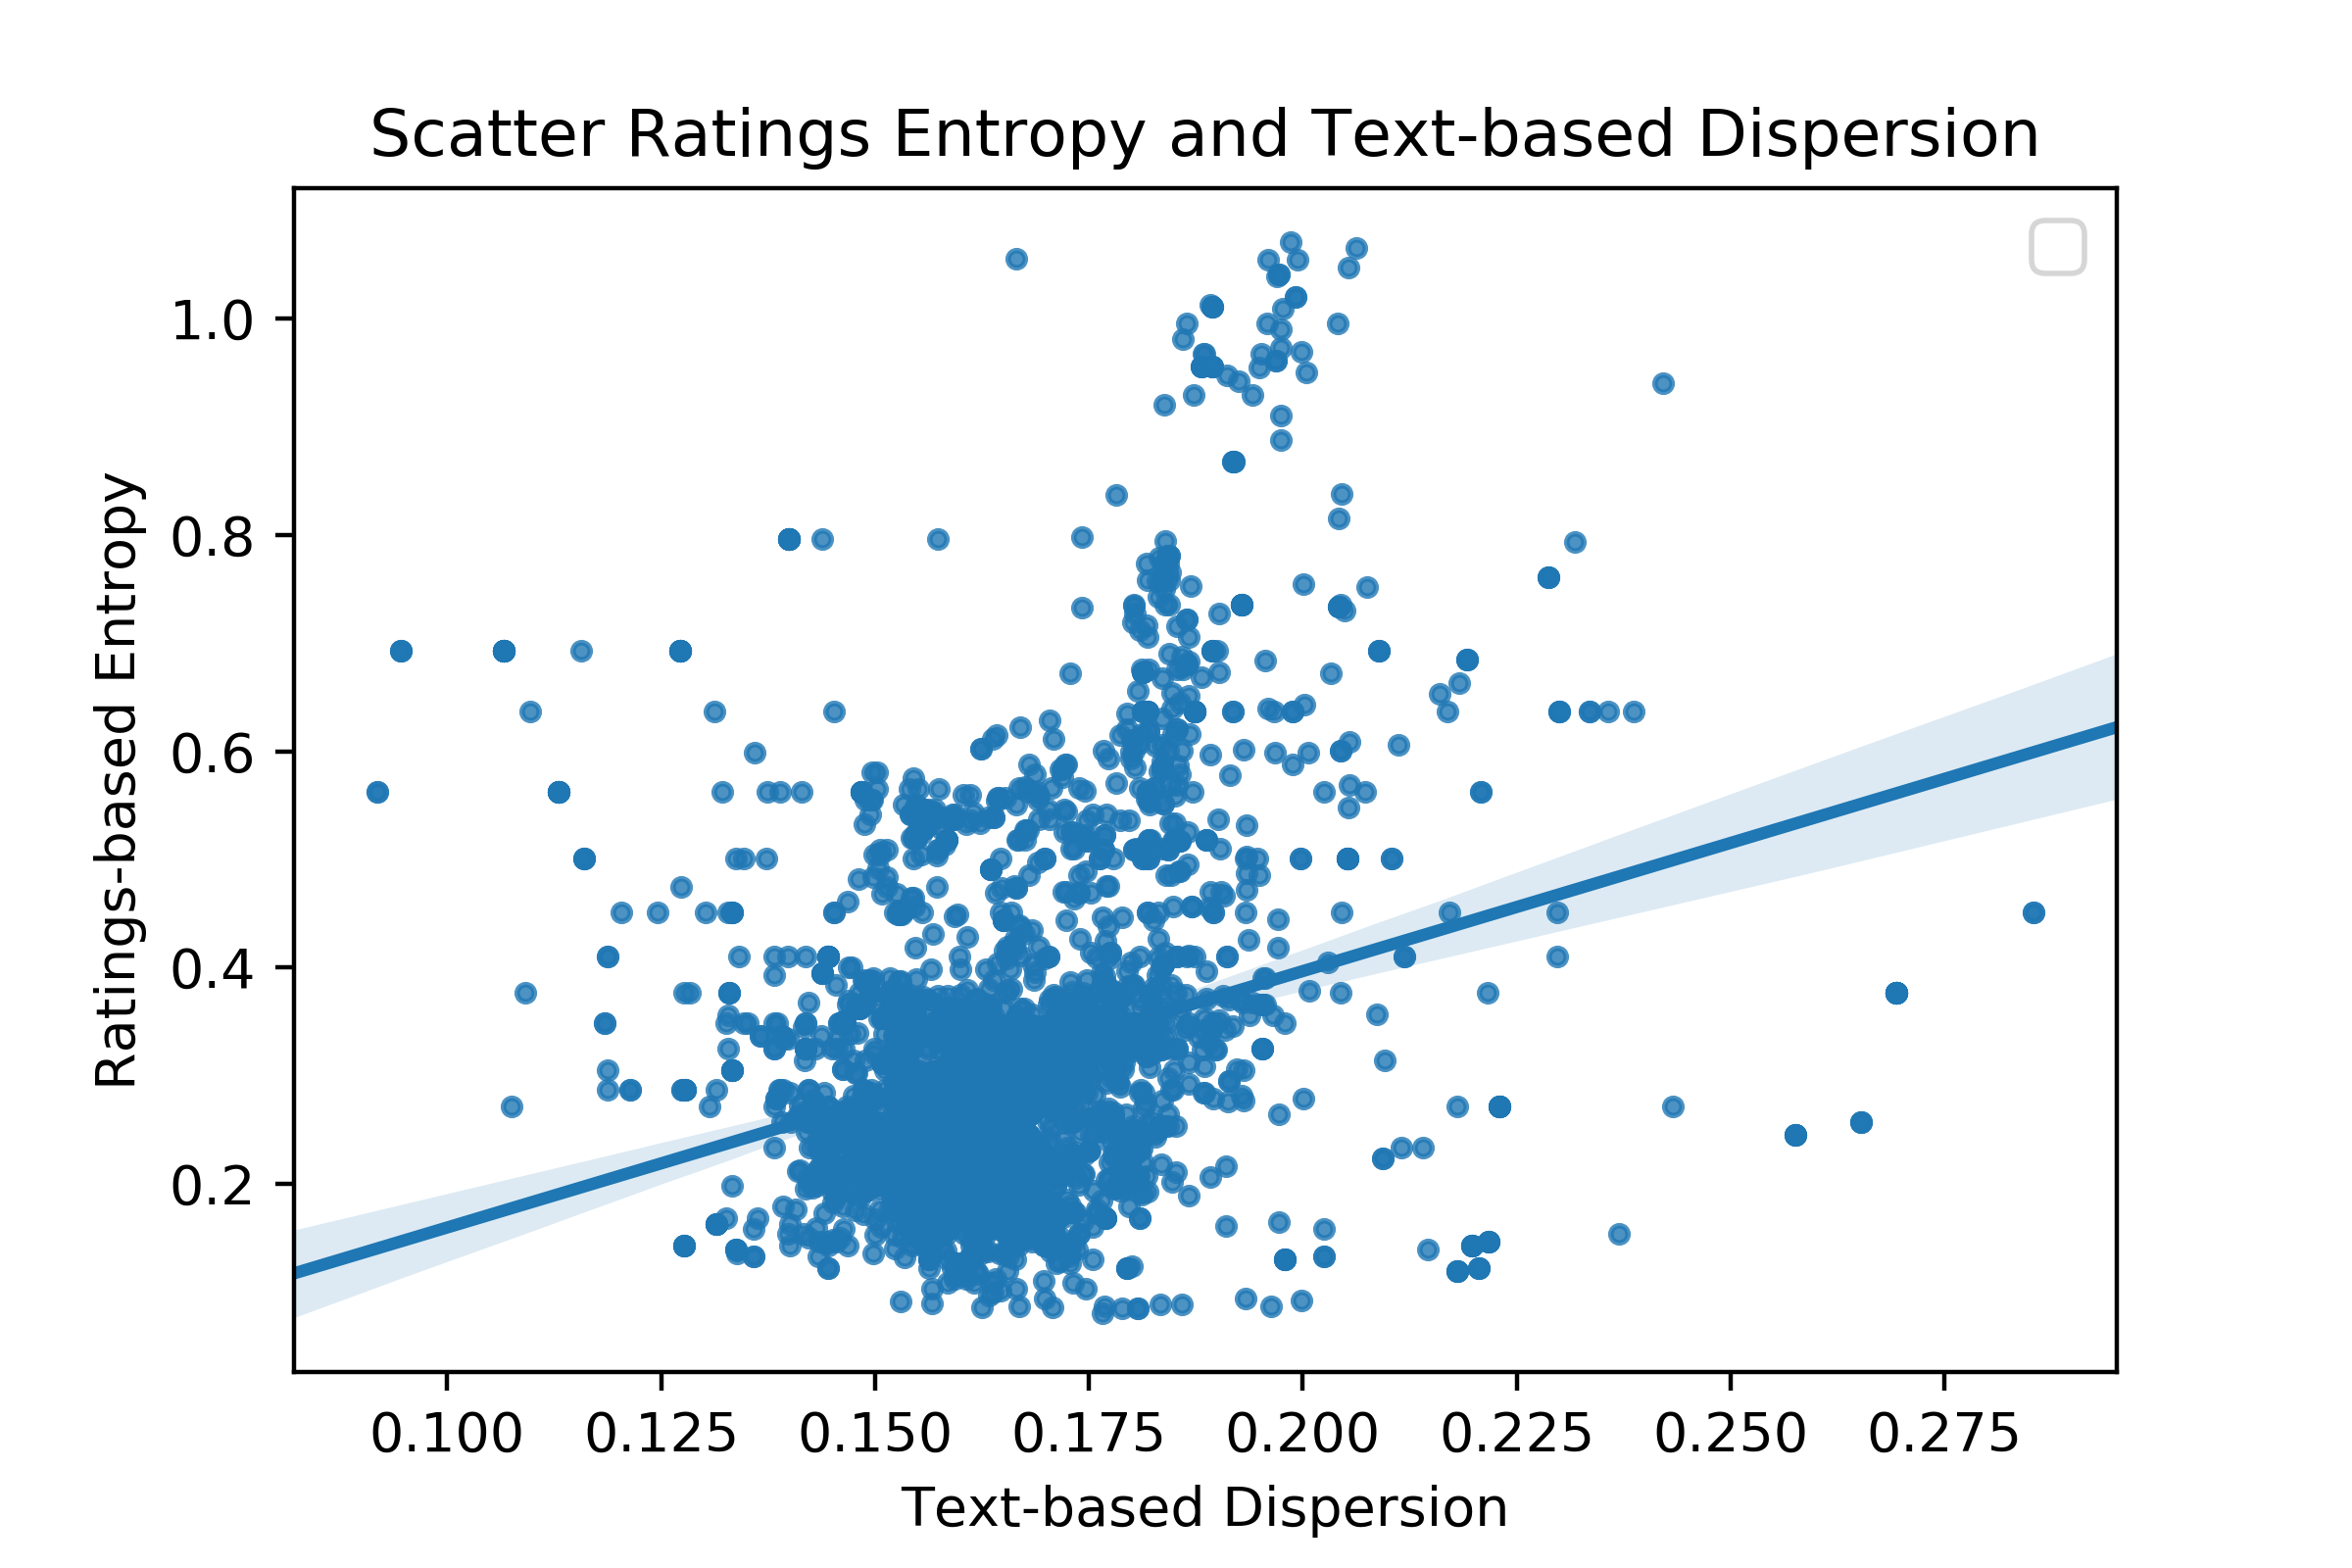
\includegraphics[width=0.7\linewidth]{regplot_text_d_ent_others.png}
	\caption{Text-based Dispersion and Entropy of Ratings}
	\label{fig: regplot_text_d_ent_others}
\end{figure}
\section{Robustness Check}
\subsection{Endogeneity}

We devised several empirical strategies to mitigate the potential drawbacks of endogeneity or omitted variables in our analysis. Regarding the individual level analysis, endogeneity could occur if there are unobserved factors that is significantly correlated with ratings dispersion that is also correlated with the activity intensities.\\
Consider that we omitted a variable that captures installer professionalism or motivation, which we denote as $pro_{i,t}$. The actual function should be

\begin{align}  \nonumber
\text{Installer\_Activity}_{i,m,t+1}=&\beta_{0}+\delta \text{pro}_it+\beta_{1} \text{Rating\_Entropy\_Self}_{i,t}+\beta_{2} \text{Rating\_Entropy\_Self}_{i,t}^ {2}
\\ \nonumber
&+\beta_{3} \text{Rating\_Entropy\_Others}_{i,t}  +\beta_{4}\text{Rating\_Entropy\_Others}_{i,t}^{2} \\
&+ \text{Controls}_{i,m,t}+ \alpha_{i} + \epsilon_{i,t+1}.
\end{align}

We argue that $pro_{it}$ would be \textit{negatively} correlated with reviews dispersion -- professional installers would be more motivated than others to deliver consistent products and services (CITE some thing).  \\

In this case, the presence of omitted variable deflated the estimates of $\beta$ (CITE ECONOMETRIC). \\


\subsection{Robustness with different local market division}
Although many similar studies used ZIP code to difine local markets(cite something from IO), we used unsupervised algorithm (OPTICS) to determine the market grouping. OPTICS algorithm requires a few parameter inputs: X, Y and Z. We used parameter XX after performing grid-search on a parameter space XXX and use Calinski-Harabasz Index to assess the appropriateness of the clustering.  \\ In addition, we used 4 digit ZIP code to define a market and the results are consistent ( INSERT RESULTS); we also use other OPTICS parameter and the results are consistent.  \\

\subsection{Dynamic Panel model}
In our main analysis we include fixed effect for each installer to account for time invariant factors. We use a dynamic panel model to perform robustness check. The inclusion of lagged dependent variables ( Activity Intensity) aim to control for unobserved heterogeneity that may influence changes in the dependent variable and is time variant. For individual level estimation, the equation we estimate is changed into the following:

\begin{align} \nonumber
\text{Installer\_Activity}_{i,m,t+1}=&\beta_{0}+\gamma_{0} \text{Installer\_Activity}_{i,t}+\gamma_{1}\text{Installer\_Activity}_{i,t-1}+\\ \nonumber
\beta_{1} \text{Rating\_Entropy\_Self}_{i,t}+\beta_{2} \text{Rating\_Entropy\_Self}_{i,t}^ {2}
&+\beta_{3} \text{Rating\_Entropy\_Others}_{i,t}  +\beta_{4}\text{Rating\_Entropy\_Others}_{i,t}^{2} \\
&+ \text{Controls}_{i,m,t}+ \epsilon_{i,t+1}.
\end{align}
The inclusion of the lagged dependent variable is to try to control for unobserved heterogeneity that may influence changes in the dependent variable, but doing so may introduce a correlation between the regressors and the error. In 1991, Arellano and Bond proposed a generalized method of moments approach to address these issues. We use their approach here. The inclusion of two lagged variables was determined so that the residuals are no long autocorrelated on the 2nd order. 
 
 
Likewise, we modify the market level model to include a lagged dependent variable $\text{Market\_Transaction}_{m,t-1}$\\
\begin{align} \nonumber&
\text{Market\_Transaction}_{m,t+1}=\beta_{5}+\gamma \text{Market\_Transaction}_{m,t}+\gamma_{1}\text{Market\_Transaction}_{m,t-1}+\\\nonumber&
\gamma_{2} \text{Market\_Transaction}_{m,t-2}+\beta_{6}\text{Rating\_Entropy\_Mkt}_{m,t}+ \beta_{7}\text{Rating\_Entropy\_Mkt}_{m,t} ^2\\\nonumber
&+ \text{Controls}_{m,t}  +\epsilon_{m,t+1}.
\end{align}
\clearpage
% Please add the following required packages to your document preamble:
% \usepackage{booktabs}
% \usepackage{graphicx}
\begin{table}[H]
\centering
\begin{tabular}{@{}lcccc@{}}
	\toprule
	& (I)            & (II)           & (III)          & (IV)           \\
	& Installer's    & Installer's    & Installer's    & Installer's    \\
	Variables                                & Activity Level & Activity Level & Activity Level & Activity Level \\ \midrule
	Installer\_Activity$_t$                 & 0.510***       & 0.507***       & 0.509***       & 0.502***       \\
	& (0.000)        & (0.000)        & (0.000)        & (0.000)        \\
	Installer\_Activity$_{t-1}$       & 0.0393         & 0.0374         & 0.0363         & 0.0369         \\
	& (0.130)        & (0.155)        & (0.176)        & (0.158)        \\
	Rating\_Entropy\_Self                    &                &                & 1.322**        & 1.351**        \\
	&                &                & (0.006)        & (0.004)        \\
	Rating\_Entropy\_Self$^2$ &                &                & -1.578*        & -1.740*        \\
	&                &                & (0.043)        & (0.026)        \\
	Rating\_Entropy\_Others           &                & 0.733          &                & 0.695          \\
	&                & (0.059)        &                & (0.069)        \\
	Rating\_Entropy\_Others$^2$       &                & -1.300*        &                & -1.253*        \\
	&                & (0.041)        &                & (0.031)        \\
	Average\_Rating\_Self                    & -0.0618***     & -0.0713***     & -0.0662***     & -0.0680***     \\
	& (0.000)        & (0.000)        & (0.000)        & (0.000)        \\
	Average\_Rating\_Others                  & -0.180         & -0.191         & -0.137         & -0.162         \\
	& (0.128)        & (0.138)        & (0.232)        & (0.183)        \\
	Review\_Count                            & 0.0165*        & 0.0175**       & 0.0134*        & 0.0105         \\
	& (0.023)        & (0.007)        & (0.024)        & (0.077)        \\
	Experience                               & -0.0554        & -0.0445        & -0.0564        & -0.0528        \\
	& (0.333)        & (0.424)        & (0.304)        & (0.326)        \\
	Price\_Difference                        & -0.0164        & 0.110          & 0.0736         & 0.0987         \\
	& (0.879)        & (0.324)        & (0.457)        & (0.366)        \\
	Market\_LogRevenue                       & 0.00348        & 0.00349        & 0.00367        & 0.00283        \\
	& (0.606)        & (0.618)        & (0.593)        & (0.681)        \\
	Observations                             & 3757           & 3757           & 3757           & 3757           \\ \bottomrule
\end{tabular}%
\begin{tablenotes}
\item Note: $p$-value in parentheses; $^\star p<0.05;^{\star\star} p<0.01;^{\star\star\star} p<0.001$
\end{tablenotes}
\vspace{10pt}
\caption{Robustness Check - Installer Level Dynamic Panels}
\label{rob_ind_dynamic}
\end{table} 
% Please add the following required packages to your document preamble:
% \usepackage{booktabs}
% \usepackage{graphicx}
\begin{table}[H]
\centering
\begin{threeparttable}[t]
\begin{tabular}{@{}lcc@{}}
\toprule
                         & (I)            & (II)           \\
                         & Market Transaction       & Market Transaction       \\
Variables                &   &   \\ \midrule
Rating\_Entropy\_Mkt     & 1.501***       & 0.751*         \\
                         & (0.000)        & (0.016)        \\
Rating\_Entropy\_Mkt$^2$ & -2.456***      & -1.609***      \\
                         & (0.000)        & (0.000)        \\
Average\_Rating\_Mkt     & -0.207         & -0.141         \\
                         & (0.169)        & (0.476)        \\
Average\_Experience      & 0.0102         & -0.00118       \\
                         & (0.157)        & (0.882)        \\
Price\_Difference\_Mkt   & 0.0349         & -0.313         \\
                         & (0.865)        & (0.089)        \\
Market\_LogRevenue       & -0.0264        & 0.0403         \\
                         & (0.502)        & (0.051)        \\
Market\_Transaction$_{t}$&                & 0.0238         \\
                         &                & (0.685)        \\
Market\_Transaction$_{t-1}$    &                & -0.00533       \\
                         &                & (0.917)        \\
Market\_Transaction$_{t-2}$   &                & 0.198**        \\
                         &                & (0.001)        \\
Market Fixed Effect      & Yes            & No             \\
Weighted State Dummies   & Yes            & Yes            \\
%Constant                 & 2.176**        &                \\
%                         & (0.003)        &                \\
Observations             & 642            & 421            \\ \bottomrule
\end{tabular}%
\begin{tablenotes}
\item Note: $p$-value in parentheses; $^\star p<0.05;^{\star\star} p<0.01;^{\star\star\star} p<0.001$
\end{tablenotes}
\end{threeparttable}
\vspace{10pt}
\caption{Robustness Check - Market Level Dynamic Panels}
\label{rob_mkt_dynamic}
\end{table} 

\subsection{Market Level Alternative Measure of Success}
% Please add the following required packages to your document preamble:
% \usepackage{booktabs}
\begin{table}[]
\centering
\begin{tabular}{@{}lccc@{}}
\toprule
 & (1) & (2) & (3) \\ \midrule
 & F.Activity & F.Activity & F.Activity \\
Entropy & 4.189** & 4.290** &  \\
 & (0.003) & (0.004) &  \\
Entropy \# Entropy & -4.066* & -4.147* &  \\
 & (0.020) & (0.018) &  \\
Text-based Entropy &  &  & 20.57 \\
 &  &  & (0.348) \\
Text-based Entropy \# Text-based Entropy &  &  & -61.58 \\
 &  &  & (0.332) \\
Rating Avg & -0.218 &  &  \\
 & (0.695) &  &  \\
Sentiment Score &  & -0.217 & 0.349 \\
 &  & (0.651) & (0.601) \\
Mkt Revenue & -0.282** & -0.288** & -0.379** \\
 & (0.008) & (0.004) & (0.005) \\
Mkt Revenue \# Mkt Revenue & 0.0158* & 0.0161** & 0.0214** \\
 & (0.014) & (0.007) & (0.008) \\
Experience(Avg) & 0.0559* & 0.0573* & 0.0740** \\
 & (0.017) & (0.013) & (0.002) \\
Price Diff(Avg) & 0.0970 & -0.00130 & -0.000982 \\
 & (0.832) & (0.998) & (0.998) \\
Constant & 6.594* & 5.596*** & 3.642 \\
 & (0.019) & (0.000) & (0.053) \\
Observations & 746 & 767 & 961 \\
p-values in parentheses &  &  &  \\
="* p\textless{}0.05 & ** p\textless{}0.01 & *** p\textless{}0.001" &  \\ \bottomrule
\end{tabular}
\caption{Market Level Use Given Quotes( instead of winning quotes) }
\label{reg_mkt_3}
\end{table}
In the analysis of ratings dispersion on local market level performance, we used total quotes accepted by consumers to measure the success of marketplace. We present results using total quotes given out by installers, and it remains consistent, as table \ref{reg_mkt_3} shows.

\subsection{Text-based Dispersion measure}
% Please add the following required packages to your document preamble:
% \usepackage{booktabs}
\begin{table}[]
\centering
\begin{tabular}{@{}lll@{}}
\toprule
 & (1) & (2) \\ \midrule
 & F.Activity & F.Activity \\
Text-based Entropy Others & 31.75* & 4.758 \\
 & 0 & -0.675 \\
Text-based Entropy Others $^2$ & -103.5* & -18.55 \\
 & 0 & -0.644 \\
Text-based Entropy (self) &  & 13.16 \\
 &  & -0.284 \\
Text-based Entropy (self)$^2$ &  & -37.23 \\
 &  & -0.246 \\
Avg Sentiment Score & -0.825* & -1.082+ \\
 & -0.027 & -0.05 \\
Avg Sent(Others) & -0.199 & -0.221 \\
 & -0.445 & -0.404 \\
Reviews Count & 0.0484* & 0.0483* \\
 & 0 & 0 \\
Experience & 0.236* & 0.0946 \\
 & -0.002 & -0.282 \\
Price Diff & -0.0598 & 0.0299 \\
 & -0.38 & -0.884 \\
Market Revenue & -0.0163* & -0.0159+ \\
 & -0.012 & -0.073 \\
Constant & 0.166 & 1.367 \\
 & -0.776 & -0.404 \\
Observations & 6210 & 3479 \\
p-values in parentheses &  &  \\
="+ p\textless{}0.10 & * p\textless{}0.05" &  \\ \bottomrule
\end{tabular}
\caption{Robustness Individual with Text-based Dispersion from Mean Distance}
\label{reg_ind_42}
\end{table}
We used median of cosine distances for measure of dispersion. The mean of cosine distances are consistent, per table \ref{reg_ind_42}.
\subsection{Excluding Inactive Installers}
Although we do not explicitly model the process of installers exiting platform, we are aware of its potential to drive results. We ran a robustness check excluding installers that have been inactive for two month ( making 0 proposals), with results presented in table \ref{rob_exclude_inactive}. The first two columns are results excluding these said installers ( cluster standard errors on market level - column (1); individual level - column (2)) . The results are virtually unchanged, especially on the independent variable of interests.
% Please add the following required packages to your document preamble:
% \usepackage{booktabs}
% \usepackage{graphicx}
\begin{table}[]
\centering
\begin{threeparttable}[t]
\begin{tabular}{@{}lccc@{}}
\toprule
                                                     & (I)            & (II)           & (III)          \\ 
                                                     & Installer's    & Installer's    & Installer's    \\
Variables                                            & Activity Level & Activity Level & Activity Level \\ \midrule
Rating\_Entropy\_Self                                &                &                & 1.428***       \\
                                                     &                &                & (0.000)        \\
Rating\_Entropy\_Self$^2$                            &                &                & -2.590***      \\
                                                     &                &                & (0.000)        \\
Rating\_Entropy\_Others                              &                & 0.386          & 0.358          \\
                                                     &                & (0.085)        & (0.108)        \\
Rating\_Entropy\_Others$^2$                          &                & -2.243***      & -2.312***      \\
                                                     &                & (0.000)        & (0.000)        \\
Average\_Rating\_Self                                & -0.551**       & -0.524*        & -0.489*        \\
                                                     & (0.007)        & (0.011)        & (0.033)        \\
Average\_Rating\_Others                              & 0.00733        & 0.000713       & 0.0000629      \\
                                                     & (0.741)        & (0.977)        & (0.998)        \\
Review\_Count                                        & 0.0504***      & 0.0479***      & 0.0436***      \\
                                                     & (0.000)        & (0.000)        & (0.000)        \\
Experience                                           & 0.136*         & 0.134*         & 0.133*         \\
                                                     & (0.010)        & (0.012)        & (0.012)        \\
Price\_Difference                                    & 0.188*         & 0.200*         & 0.208*         \\
                                                     & (0.036)        & (0.027)        & (0.021)        \\
Market\_LogRevenue                                   & -0.00645       & -0.00618       & -0.00553       \\
                                                     & (0.148)        & (0.165)        & (0.216)        \\
Constant                                             & 2.788***       & 2.868***       & 2.995***       \\
                                                     & (0.000)        & (0.000)        & (0.000)        \\
Fixed Effect                                         & Yes            & Yes            & Yes            \\
State Dummies                                        & Yes            & Yes            & Yes            \\
Observations                                         & 3472           & 3472           & 3472           \\
Adjusted R$^2$                                          & 0.622          & 0.625          & 0.627          \\
AIC                                                  & 9693.2         & 9670.1         & 9655.4         \\
BIC                                                  & 9748.6         & 9737.7         & 9735.3         \\ \bottomrule
\end{tabular}%
\begin{tablenotes}
\item Note: $p$-value in parentheses; $^\star p<0.05;^{\star\star} p<0.01;^{\star\star\star} p<0.001 $
\end{tablenotes}
\caption{Robustness Check Excluding Inactive Installers}
\end{threeparttable}
\label{rob_exclude_inactive}
\end{table}

\section{Discussions}

\paragraph{Average Ratings and Sentiment} : Most the specifications concerning the impact of average ratings captured negative (yet statistically insignificant) effects.  Interestingly, the model using sentiment score and Text-based dispersion measures (table \ref{reg_ind_withtext}) have shown more consistent and significant negative coefficients. After we control for other things, being rated higher or viewed more positive is associated with a lower level of activity intensity going forward. \\

\paragraph{Noise in Reviews} The individual level analysis pertain to ratings and reviews dispersion all revealed an inverted-U type of impact.

\paragraph{Noisy Reviews and Marketplace Matching Performance}: from the marketplace's perspective, dispersion in reviews also exhibits an inverted-U type of relationship with market place matches.

\paragraph{Methodology - text mining} To analyze the reviews texts, we incorporated two text mining methods that 1) - gave reviews texts a one-dimensional sentiment score and 2) utilize word embedding model to measure texts similarity with precision. We demonstrated that the text mining tools are great complement to the quantitative data. To our knowledge, it is the first example of using deep learning based text-mining models on business settings in the operations management literature. We demonstrate the versatility of deep learning methods as a complement to traditional text-mining methods.
\begin{APPENDIX}{Note and Questions for Our Own References }
% Please add the following required packages to your document preamble:
% \usepackage{booktabs}
\begin{table}[]
\centering
\begin{tabular}{@{}lll@{}}
\toprule
Variable                           & VIF  & 1/VIF \\ \midrule
Rating\_Entropy\_Self                & 7.10 & 0.14  \\
Rating\_Entropy\_Self$^2$            & 5.81 & 0.17  \\
Rating\_Entropy\_Others              & 1.83 & 0.55  \\
Rating\_Entropy\_Others$^2$          & 1.46 & 0.68  \\
Average\_Rating\_Self                & 4.59 & 0.22  \\
Average\_Rating\_Others             & 1.40 & 0.71  \\
Reviews\_Count                      & 1.24 & 0.81  \\
Experience                         & 1.46 & 0.68  \\
Price\_Difference                  & 1.03 & 0.97  \\
Market\_LogRevenue                 & 1.65 & 0.61  \\ \bottomrule
\end{tabular}
\caption{VIF table: Installer Level}
\label{vif_ind}
\end{table}
% Please add the following required packages to your document preamble:
% \usepackage{booktabs}
\begin{table}[H]
\centering
\begin{tabular}{@{}lcc@{}}
\toprule
Variable           & VIF  & 1/VIF    \\ \midrule
Rating\_Entropy\_Mkt    & 6.67 & 0.149965 \\
Rating\_Entropy\_Mkt$^2$ & 6.21 & 0.160950 \\
Average\_Rating\_Mkt     & 1.58 & 0.632615 \\
Experience     & 1.46 & 0.685113 \\
Price\_Difference   & 1.01 & 0.986885 \\
Market\_LogRevenue     & 1.45 & 0.690279 \\ \bottomrule
\end{tabular}
\caption{VIF Table:Market level}
\label{vif_mkt}
\end{table} 
% Please add the following required packages to your document preamble:
% \usepackage{booktabs}
\begin{table}[H]
\centering
\begin{tabular}{@{}ccc@{}}
\toprule
\multicolumn{1}{l}{\textbf{Installer Level Dynamic Panel}} & \multicolumn{1}{l}{} & \multicolumn{1}{l}{} \\ \midrule
Order                                   & z                    & $p-value$  \\
$H_{0}$: No correlation between $\Delta_{i,t}$ and $\Delta_{i,t-1}$ & -9.8283  & 0.00 \\
$H_{0}$: No correlation between $\Delta_{i,t}$ and $\Delta_{i,t-2}$  & -0.66053 & 0.5089 \\
 Sargan Test for overidentifying restriction & $\chi^2(1525)$  =  238.2181& 1.000 \\ \midrule
\textbf{Market Level Dynamic Panel}          &    &      \\ \midrule
Order                           & z      & $p-value$  \\
$H_{0}$: No correlation between $\Delta_{i,t}$ and $\Delta_{i,t-1}$  & -2.7882 & 0.01 \\
$H_{0}$: No correlation between $\Delta_{i,t}$ and $\Delta_{i,t-2}$  & 0.04295  & 0.9657 \\
 Sargan Test for overidentifying restriction & $\chi^2(544)$ =  22.77427 & 1.000 \\ \bottomrule
\end{tabular}
\caption{Dynamic Panel Specification Checks
}
\label{autocorrelation_test}
\end{table} 
\section{Tests for Fixed and Random Effects in \eqref{model_ind_3}}\ref{Apx: Hausman}
\label{Apx: Hausman}
 Individual Level - FE vs RE Hausman 
 Test:  Ho:  difference in coefficients not systematic

$chi2(13) = (b-B)'[(V_b-V_B)^(-1)](b-B)$\\
$=       44.23$\\
$Prob>chi2 =      0.0000$\\

Market Level -FE vs. RE Hausman\\
 Test:  Ho:  difference in coefficients not systematic

$chi2(18) = (b-B)'[(V_b-V_B)^(-1)](b-B)
=      403.30
Prob>chi2 =      0.0000$ 
\textbf{PLEASE INSERT A TABLE THAT REPORTS THE TEST RESULTS}



\section{My Earlier Question}

What is the total number of proposals in each year?
Which state is number \#1 in terms of total wins/total proposals?
Which state is worst in terms of total wins/total proposals?
Q1) IF THEY OPERATE AT MULTIPLE LOCATIONS, DO THEY PROVIDE
THAT INFO ON THEIR PROFILE? \\
We do not have info if they operated on multiple locations or not. I scrape their headquarter address , with ZIP code info.
Q2) WHAT IS THE FORMAT OF THE LOCATION INFO - IS IT A DETAILED
ONE WITH A ZIPCODE? PLEASE INCLUDE AN EXAMPLE FOR ME HERE. \\
Emerald Energy of North Carolina Headquarters
2624 Leighton Ridge Drive, Suite 120
Wake Forest, NC
27587 US

COULD YOU PLEASE PREPARE THESE TWO GRAPHS? 1) TOTAL NUMBER
OF REVIEWS PER INSTALLER - MAX NUMBER OF REVIEW FOR AN IN-
STALLER AND HISTOGRAM? 2) NUMBER OF INSTALLERS IN EACH STATE
FOR TOP 10 STATES \\
QUESTIONS: 1) HOW MANY OF THE INSTALLERS DO NOT HAVE A RE-
VIEW? 2) WHAT IS THE PERCENTAGE OF THOSE INSTALLERS IN THE LO-
CAL MARKET WIN AND SUBMITTED PROPOSALS? 3) WHAT DO YOU AS-
SUME ABOUT THEM IN THE EMPIRICAL ANALYSIS? \\
We didn't need to assume anything. I just computed all the variables the way as we stated. \\
All installers started with 0 reviews, naturally. \\
If we look at the observations that are included in the analysis, less than 5 percent of observations have 0 reviews ( mostly due to its newly established). \\
If we look at the end of the panel, only 1 installer has 0 reviews, and have a positive entothers value ( hence is included in the analysis)



\textbf{YOU MENTIONED controls are to capture factors that are irrelevant to the rating entropy. Is Experience really irrelevant to the rating entropy?? }

\end{APPENDIX}


\clearpage
% Appendix here
% Options are (1) APPENDIX (with or without general title) or
%             (2) APPENDICES (if it has more than one unrelated sections)
% Outcomment the appropriate case if necessary
%
% \begin{APPENDIX}{<Title of the Appendix>}
% \end{APPENDIX}
%
%   or
%
% \begin{APPENDICES}
% \section{<Title of Section A>}
% \section{<Title of Section B>}
% etc
% \end{APPENDICES}


% Acknowledgments here
\ACKNOWLEDGMENT{ .}


% References here (outcomment the appropriate case)

% CASE 1: BiBTeX used to constantly update the references
%   (while the paper is being written).
%\bibliographystyle{informs2014} % outcomment this and next line in Case 1
%\bibliography{<your bib file(s)>} % if more than one, comma separated

% CASE 2: BiBTeX used to generate mypaper.bbl (to be further fine tuned)
%\input{mypaper.bbl} % outcomment this line in Case 2

%If you don't use BiBTex, you can manually itemize references as shown below.


\bibliographystyle{informs2014} % outcomment this and next line in Case 1
\bibliography{solarlits} % if more than one, comma separated


%%%%%%%%%%%%%%%%%
\end{document}
%%%%%%%%%%%%%%%%%

